\documentclass[a4paper,12pt]{report}
\usepackage{amssymb,amsfonts,amsmath,amsthm,dsfont,vmargin, mathtools, braket}
\usepackage{graphicx, booktabs, caption, subfig, float, wrapfig, pgfplots}
\usepackage[output-decimal-marker={,}]{siunitx}
\usepackage{microtype, tikz}
\usepackage[europeanvoltages,americancurrents]{circuitikz}
\usepackage[T1]{fontenc}
\usepackage{lmodern} %� un font scalabile, indispensabile per pdfLaTeX se si usa il pacchetto microtype
\usepackage[latin1]{inputenc}
\usepackage[italian]{babel}
\usepackage{natbib}
\usepackage{hyperref}
\usetikzlibrary{calc}
%\usepackage{color}
%\usepackage{transparent}
%\usepackage{pstricks}

\DeclareMathOperator{\dB}{dB}
\DeclareMathOperator{\dec}{dec}
\DeclareMathOperator{\dBd}{dB/dec}
\DeclareMathOperator{\sgn}{sgn}
\DeclarePairedDelimiter{\abs}{\lvert}{\rvert}
\newcommand{\Arg}[1]{\phase\left(#1\right)}
\newcommand{\Logb}[1]{\log_{10}\left(#1\right)}

\newcommand{\numberset}{\mathbb}
\newcommand{\R}{\numberset{R}}
\newcommand{\OL}[1]{\overline{#1}}
\newcommand{\I}{\overline{I}}
\newcommand{\V}{\overline{V}}
\newcommand{\Epsilon}{\mathcal{E}}
\newcommand{\lap}{\mathcal{L}}
\newcommand{\Par}{{//}}
\newcommand{\Th}{{TH}}
\newcommand{\No}{{NO}}
\newcommand{\phase}{\measuredangle}
\newcommand{\Log}{{\log_{10}}}

\setpapersize{A4}

\theoremstyle{plain}
\newtheorem{teorema}{Teorema} [section]

\theoremstyle{definition}
\newtheorem{dfn}{Definizione} [section]
\newtheorem{obs}{Osservazione} [section]

\newtheorem{examplex}{Esempio} [section]
\newenvironment{example}
  {\pushQED{\qed}\renewcommand{\qedsymbol}{$\clubsuit$}\examplex}
  {\popQED\endexamplex}

\newfloat{Circuito}{htbp}{loc}[chapter]
\newsubfloat{Circuito}

\begin{document}

\author{Simone Laierno}
\title{Appunti di Elettronica}
\maketitle
\tableofcontents

\chapter{Richiami di teoria sulle reti elettriche}

Questo capitolo vuole essere un riassunto della teoria sulle reti elettriche per chi da molto tempo � lontano dal mondo dei circuiti elettrici o per chi vuole avere un ripasso generale di nozioni gi� note.
Si invita quindi il lettore esperto a saltare questo capitolo ed utilizzarlo solo come <<formulario>> di concetti gi� noti.

\section{Componenti passivi e generatori}

\subsection{Componenti passivi}

I componenti passivi basilari utilizzati nelle reti elettriche sono i seguenti:

\begin{itemize} 
	\item Resistori
			\footnote{Resistori e induttori sono comunemente detti <<resistenze>> e <<induttanze>> ma non sono da confondere con le unit� di misura dei componenti stessi.}
	\item Condensatori
	\item Induttori $^1$
\end{itemize}

Tali componenti mettono in relazione la differenza di potenziale $V$ e la corrente $I$ tramite le seguenti relazioni:
\begin{itemize} %Elenco componenti
	\item Resistore \\
		 $$V=RI \qquad [R]=\Omega$$
		\begin{center}
			\begin{circuitikz}
			\draw (0,0) to [R=$R$, i =$I$, v<=$V$] (2,0);
			\end{circuitikz}
		\end{center}

	\item Condensatore \\
		 $$I=C\frac{dV}{dt} \qquad [C]=F$$
		  \begin{center}
			\begin{circuitikz}
			\draw (0,0) to [C=$C$, i =$I$, v<=$V$] (2,0);
			\end{circuitikz}
		 \end{center}
	\item Induttore \\
		 $$V=L\frac{dI}{dt} \qquad [L]=H$$
		  \begin{center}
			\begin{circuitikz}
			\draw (0,0) to [L=$L$, i =$I$, v<=$V$] (2,0);
			\end{circuitikz}
		  \end{center}
\end{itemize}

Le relazioni $V-I$ per i condensatori e gli induttori, a differenza della relazione lineare $V=RI$ ben nota come \textit{Legge di Ohm}, sono integro-differenziali e di conseguenza pi� difficili da gestire matematicamente. Si vedr� tra breve come comportarsi per tali componenti in situazioni particolari ma di largo utilizzo.

\subsection{Generatori indipendenti}

I \textit{generatori indipendenti} sono generatori di corrente o di tensione che non dipendono da altre grandezze del circuito. Rispettivamente, generano una corrente costante in un ramo ed una differenza di potenziale costante tra due nodi.
Faremo distinzione tra generatori in \emph{DC} o \emph{in continua}, che generano una corrente o una differenza di potenziale \textit{costante}, e generatori \textit{di segnale}, che generano un segnale di tensione o di corrente sinusoidale.

\begin{itemize} %Elenco di generatori

	\item \textbf{Generatori in continua}\\ \\
	\begin{circuitikz}
			\draw (0,0) to [battery1] (2,0);
	\end{circuitikz}
	Generatore di tensione
	\begin{circuitikz}
			\draw (0,0) to [I] (2,0);
	\end{circuitikz}
	Generatore di corrente
	
	\item \textbf{Generatori di segnale}\\ \\
	\begin{circuitikz}
			\draw (0,0) to [sV] (2,0);
	\end{circuitikz}
	Generatore di tensione
	\begin{circuitikz}
			\draw (0,0) to [I] (2,0);
	\end{circuitikz}
	Generatore di corrente
	
\end{itemize}

I generatori di tensione si compongono \emph{in serie} mentre i generatori di corrente si compongono \emph{in parallelo}:\\

\begin{circuitikz} %composizione serie
	\draw
	(0,0) node {}
	(0,0.5) node[anchor=north] (A) {}
		to[short,o-] (0,1.5)
		to[battery1, l=$E$] (2,1.5)
		to[sV, l=$V_i$] (4,1.5)
	(4,1.5) to[short,-o] (4,0.5)
	(4,0.5) node[anchor=north] (B) {}
	(A) to[open,v=$V_x$] (B)
	(5.5,1) node {$V_x=E+V_i$}
	(8,0) node[anchor=east] (X) {}
	(9,0) to[short,i=$I_x$, -o] (8,0)
	(9,2) to[I, l=$I$] (9,0)
	(9,2) -- (11,2) to[I, l=$i$] (11,0) -- (9,0)
	(8,2) to[short,o-, i=$I_x$] (9,2)
	(8,2) node[anchor=east] (Y) {}
	(13,1) node {$I_x=I+i$}
;\end{circuitikz}

\subsection{Generatori pilotati o dipendenti}

I generatori, sia di tensione che di corrente, possono non essere indipendenti ed essere in realt� dei componenti che generano una differenza di potenziale tra due nodi o una corrente in un ramo \emph{in funzione di altre grandezze nel circuito}.
Tali componenti sono detti \emph{generatori pilotati} o \emph{dipendenti}.

\begin{itemize}
	\item \emph{Generatore di tensione controllato in tensione}
	\begin{center} %circuito
	\begin{circuitikz}
	\draw
		(0,0) node[anchor=east] (B) {}
			to[short, o-] (1.5,0) 
		(0,2) node[anchor=east] (A) {}
			to[short, o-] (1.5,2)
		(4.5,0) node[anchor=west] (D){}
			to[short, o-] (2.5,0)
			to[battery1,l] (2.5,2)
			to[short, -o] (4.5,2) node[anchor=west] (C) {}
		(A) to[open, v=$V_i$] (B)
		(C) to[open, v^=$V_0{=}A\cdot V_i$] (D);
		\draw [dashed] (1,-0.5) -- (1,2.5) -- (4,2.5) -- (4,-0.5) -- (1,-0.5);	
	\draw (7.7,1) node[anchor=east] (E) {=};
		\draw (10,0) to [american controlled voltage source, l=$A\cdot V_i$] (10,2);		
		\end{circuitikz}
	\end{center}
	
		Un generatore di tensione controllato in tensione assume un \emph{guadagno A adimensionale}. Questo dovuto all'ovvio fatto che trasforma una tensione in un'altra tensione, non apportando modifiche all'unit� di misura.
		
		\item \emph{Generatore di corrente controllato in tensione}
	\begin{center} %circuito
	\begin{circuitikz}
	\draw
		(0,0) node[anchor=east] (B) {}
			to[short, o-] (1.5,0)
		(0,2) node[anchor=east] (A) {}
			to[short, o-] (1.5,2)
		(4.5,0) node[anchor=west] (D){}
			to[short, o-] (2.5,0)
			to[I_=$I_0{=}G\cdot V_i$] (2.5,2)
			to[short, -o] (4.5,2) node[anchor=west] (C) {}
		(A) to[open, v=$V_i$] (B) ;
		\draw [dashed] (1,-0.5) -- (1,2.5) -- (4.3,2.5) -- (4.3,-0.5) -- (1,-0.5);	
	\draw (5.7,1) node[anchor=east] (E) {=};
		\draw (8,0) to [american controlled current source=$G\cdot V_i$] (8,2);		
		\end{circuitikz}
	\end{center}
	
	Un generatore di corrente controllato in tensione assume un \emph{guadagno G} di \emph{transconduttanza} $[G]=\Omega ^{-1}$. La dimensione � l'inverso di una resistenza poich�, per la legge di Ohm, $I=\frac{V}{R}$, e quindi $[G]=[\frac{1}{R}]$.
	
	\item \emph{Generatore di tensione controllato in corrente}
	\begin{center} %circuito
	\begin{circuitikz}
	\draw
		(0,2) node[anchor=east] (A) {}
			to[short, o-] (1.5,2)
			to[I=$I_i$] (1.5,0)
			to[short, -o] (0,0) node[anchor=east] (B) {}
		(4.5,0) node[anchor=west] (D){}
			to[short, o-] (3,0)
			to[battery1] (3,2)
			to[short, -o] (4.5,2) node[anchor=west] (C) {}
		(C) to[open, v^=$V_0{=}H\cdot I_i$] (D);
		\draw [dashed] (1,-0.5) -- (1,2.5) -- (4,2.5) -- (4,-0.5) -- (1,-0.5);	
	\draw (7.7,1) node[anchor=east] (E) {=};
		\draw (10,0) to [american controlled voltage source, l=$H\cdot V_i$] (10,2);		
		\end{circuitikz}
	\end{center}
	
	Un generatore di tensione controllato in corrente assume un \emph{guadagno H} di \emph{transresistenza} $[H]=\Omega$. La dimensione � quella di una resistenza poich�, per la legge di Ohm, $V=RI$, e quindi $[H]=[R]$.
	
	\item \emph{Generatore di corrente controllato in corrente}
	\begin{center} %circuito
	\begin{circuitikz}
	\draw
		(0,2) node[anchor=east] (A) {}
			to[short, o-] (1.5,2)
			to[I=$I_i$] (1.5,0)
			to[short, -o] (0,0) node[anchor=east] (B) {}
		(4.5,0) node[anchor=west] (D){}
			to[short, o-] (3,0)
			to[I_=$I_0{=}G\cdot V_i$] (3,2)
			to[short, -o] (4.5,2) node[anchor=west] (C) {};
		\draw [dashed] (1,-0.5) -- (1,2.5) -- (4,2.5) -- (4,-0.5) -- (1,-0.5);	
	\draw (5.7,1) node[anchor=east] (E) {=};
		\draw (8,0) to [american controlled current source=$F\cdot V_i$] (8,2);		
		\end{circuitikz}
	\end{center}

Un generatore di corrente controllato in corrente assume un \emph{guadagno F adimensionale}. Come per il generatore di tensione pilotato in tensione, l'adimensionalit� del guadagno � ovvia conseguenza di una trasformazione di una grandezza in una analoga (corrente$\rightarrow$corrente).			
\end{itemize}



\section{Circuiti in regime sinusoidale}

\emph{NOTA: Questa sezione non ha pretesa di essere rigorosa n� in ambito fisico n� in ambito matematico. Vuole solo essere un richiamo delle conoscenze che si ritengono gi� acquisite dai corsi di Analisi Matematica e Fisica.}

\subsection{Metodo simbolico}
Consideriamo l'equazione differenziale lineare a coefficienti costanti di ordine $n$:
	\begin{equation} \label{eq:A}
	\sum^n_{i=0} c_i \frac{d^i y(t)}{dt^i}=f(t)
	\end{equation}
A partire da questa, consideriamo la nuova equazione differenziale aggiungendo a secondo membro la funzione $\jmath g(t)$:
	\begin{equation} \label{eq:B}
	\sum^n_{i=0} c_i \frac{d^i \upsilon (t)}{dt^i}=f(t) + \jmath g(t)
	\end{equation}
Ove la funzione $\upsilon (t)$ � in generale complessa e diversa dalla funzione $y(t)$. Possiamo pertanto esprimerla come:
	\begin{equation}
	\upsilon (t) = a(t) + \jmath b(t)
	\end{equation}
Ove:
	$$
	a(t),b(t):\R \longrightarrow \R
	$$
\\
Risulta quindi evidente che la \eqref{eq:A} pu� essere riscritta come:
	\begin{equation}
	\sum^n_{i=0} c_i \frac{d^i a(t)}{dt^i} + \jmath\sum^n_{i=0} c_i \frac{d^i b(t)}{dt^i} = f(t) + \jmath g(t)
	\end{equation}
Perci�, eguagliando parte reale e parte immaginaria:
	\begin{align}
	\sum^n_{i=0} c_i \frac{d^i a(t)}{dt^i} = f(t) \notag \\
	\sum^n_{i=0} c_i \frac{d^i b(t)}{dt^i} = g(t)
	\end{align}
Da ci� si deduce che $a(t)$ � la $y(t)$ soluzione dell'equazione originaria \eqref{eq:A} e quindi:
	\begin{equation}
	y(t)=\Re[a(t)+\jmath b(t)]
	\end{equation}
Questo metodo di risoluzione delle equazioni differenziali lineari � noto con il nome di \emph{metodo simbolico}.\\

Scegliendo in modo opportuno $f(t)$ e $g(t)$ si possono prendere in esame i casi di nostro interesse, quali sono i circuiti stimolati da un ingresso sinusoidale. \\
Supponendo $f(t)=A\cos(\omega t)$, la forma analitica di $g(t)$ sar� $g(t) = A\sin(\omega t)$. In tal modo:
	\begin{equation}
	f(t)+\jmath g(t) = A\cos(\omega t) + \jmath A\sin(\omega t) = Ae^{\jmath \omega t}
	\end{equation}
A tutti gli effetti, ci� significa che per ottenere la \eqref{eq:B} a partire dalla \eqref{eq:A} � sufficiente sostituire al termine $\cos(\omega t)$ il termine $e^{\jmath \omega t}$, risolvere l'equazione differenziale ed estrarne la parte reale.\\
\\
\emph{NOTA: A tutti gli effetti pu� essere fatto il discorso analogo prendendo come riferimento $\sin(\omega t)$ ed estrarre la parte immaginaria. Si fa notare inoltre che pu� comunque essere risolto con la parte reale ricordando l'uguaglianza:}
$$\sin(\omega t) = \cos(\pi - \omega t)$$
\emph{Per comodit� considereremo gli ingressi come funzioni di seno e calcolando la parte immaginaria delle estensioni complesse, fermo restando che si pu� applicare ogni ragionamento anche a funzioni di coseno senza perdere generalit�}

\subsection{Impedenze}

L'impedenza di un componente (o eventualmente di una rete di componenti), indicata con $Z$ � definita come:
	\begin{equation}
	Z\triangleq\frac{\V}{\I}
	\end{equation}
Cio� quel valore (eventualmente complesso) tale per cui vale la seguente relazione, detta \emph{Legge di Ohm generalizzata}
	\begin{equation}
	\V=Z\I
	\end{equation}
\\
Faremo in modo, cio�, di trattare ogni componente (o rete elettrica) come fosse una resistenza a valori eventualmente complessi.

\emph{NOTA: D'ora in poi supporremo sempre che il circuito sia stimolato sinusoidalmente e portato a regime, cio� non considereremo lo stato transitorio del circuito.}

\subsubsection{Impedenza resistiva}

Consideriamo una resistenza ai cui capi � applicata una differenza di potenziale $V$ e nella quale scorra una corrente $I$:
		\begin{center} %resistenza
			\begin{circuitikz}
			\draw (0,0) to [R=$R$, i =$I$, v<=$V$] (2,0);
			\end{circuitikz}
		\end{center}
La relazione $V-I$ �, come gi� spiegato, definita dalla \emph{legge di Ohm} $V=RI$, l'impedenza resistiva perci� vale:
	\begin{equation} \label{eq:ZR}
	Z_R=\frac{\V}{\I}=R
	\end{equation}
La resistenza non fornisce alcun problema nel caso di circuiti in regime sinusoidale, in quanto l'impedenza � il valore (reale) della resistenza del componente.


\subsubsection{Impendenza capacitiva}
Consideriamo un condensatore ai cui capi � applicata una differenza di potenziale $V$ e nella quale scorra una corrente $I$:

 		\begin{center} %condensatore
			\begin{circuitikz}
			\draw (0,0) to [C=$C$, i =$I$, v<=$V$] (2,0);
			\end{circuitikz}
		 \end{center}
		 
� noto che la relazione tra la differenza di potenziale e la corrente �:
	$$
	I=C\frac{dV}{dt}
	$$
Consideriamo il caso in cui l'ingresso sia sinusoidale del tipo:
	$$
	V=V_0\sin(\omega t)
	$$
E applichiamo il metodo simbolico alla relazione differenziale $I=C\frac{dV}{dt}$ imponendo le estensioni complesse:
	\begin{equation} 
	\V = V_0 e^{\jmath \omega t} \qquad \I=I_0 e^{\jmath \omega t} $$$$
	\I=C\frac{d\V}{dt}=C\frac{d}{dt}\left(V_0 e^{\jmath \omega t}\right)=\jmath \omega C V_0 e^{\jmath \omega t} = \jmath \omega C \V
	\end{equation}
Da ci�, l'impedenza risulta:
	\begin{equation} \label{eq:ZC}
	Z=\frac{\V}{\I} \Rightarrow Z_C = \frac{1}{\jmath \omega C}
	\end{equation}

\subsubsection{Impedenza induttiva}

Consideriamo un induttore \footnote{Si far� in realt� un uso pressoch� nullo delle induttanze in questa trattazione. L'argomento viene trattato solo per completezza.} ai cui capi � applicata una differenza di potenziale $V$ e nella quale scorra una corrente $I$

	\begin{center}	%induttore
			\begin{circuitikz}
			\draw (0,0) to [L=$L$, i =$I$, v<=$V$] (2,0);
			\end{circuitikz}
		  \end{center}

Nota la relazione $I-V$ in un'induttanza:
	$$
	V=L\frac{dI}{dt}
	$$
Assegnate le estensioni complesse come nei casi precedenti:
	$$
	\V = V_0 e^{\jmath \omega t} \qquad \I=I_0 e^{\jmath \omega t} $$
Ricaviamo in modo analogo al precedente l'impedenza di un induttore:
	\begin{equation}
	\V=L\frac{d\I}{dt}=L\frac{d}{dt}\left[I_0 e^{\jmath \omega t} \right] = \jmath \omega L I_0 e^{\jmath \omega t} = \jmath \omega L \I
	\end{equation}
Da ci�, l'impedenza induttiva:
	\begin{equation} \label{eq:ZL}
	Z=\frac{\V}{\I} \Rightarrow Z = \jmath \omega L
	\end{equation}

Spesso, nell'utilizzo delle impedenze complesse per l'analisi in frequenza, si opera la sostituzione\footnote{Il motivo di tale sostituzione sar� accennato pi� avanti.}

\begin{equation}
s=\jmath \omega
\end{equation}

E quindi le impedenze saranno espresse come:
\begin{equation}
Z_R = R \qquad Z_C = \frac{1}{sC} \qquad Z_L = sL
\end{equation}


\section{Leggi e teoremi delle reti elettriche}

\subsection{Leggi di Kirchoff}
Enunciamo senza dimostrazione le due leggi basilari delle reti elettriche, le \emph{Leggi di Kirchoff}:

\subsubsection{Legge di Kirchoff per le correnti (LKC)}

	\begin{center} %stella impedenze
	\begin{circuitikz}
	\ctikzset{label/align = smart} 
		\draw node [anchor=north] (A) {};
		\def\DIR{18/1,162/3,-126/5}
		\foreach \i/\j in \DIR {
			\draw (A) to [european resistor, i=$I_\j$,*-o] (\i :2.5);
			}
		\def\DIR{90/2,-54/4}
		\foreach \i/\j in \DIR {
			\draw (A) to [european resistor, i<=$I_\j$,*-o] (\i :2.5);
			}
	\end{circuitikz}
	\end{center}

La legge di Kirchoff per le correnti\footnote{� detta anche \emph{Legge di Kirchoff ai nodi} o \emph{Prima legge di Kirchoff}.} afferma che, dato un nodo in cui convergono $n$ correnti, prese \emph{positive} se entranti e \emph{negative} se uscenti:
	\begin{equation}
	\sum_{i=1}^n I_i=0
	\end{equation}
In termini pi� semplici:\\
\emph{La somma delle correnti entranti in un nodo � uguale alla somma delle correnti uscenti dal nodo.}
\begin{example}
Data la seguente configurazione di circuito con le correnti indicate:
	\begin{center} %stella resistenze
	\begin{circuitikz}
	\ctikzset{label/align = smart} 
		\draw node [anchor=north] (A) {};
		\def\DIR{18/10 mA,162/5 mA,-126/x}
		\foreach \i/\j in \DIR {
			\draw (A) to [european resistor, i=\j,*-o] (\i :2.5);
			}
		\def\DIR{90/6 mA,-54/12 mA}
		\foreach \i/\j in \DIR {
			\draw (A) to [european resistor, i<=\j,*-o] (\i :2.5);
			}
	\end{circuitikz}
	\end{center}
Determiniamo quindi verso e intensit� della corrente $x$, supponendo sia uscente. Nel caso in cui si sia fatta una supposizione errata, il risultato verr� negativo e quindi sar� corretto in valore assoluto e il verso sar� l'opposto di quello supposto all'inizio.
Per la prima legge di Kirchoff la somma delle correnti uscenti � uguale alla somma delle correnti entranti. Perci�:
	\begin{equation}
	10mA+5mA+x=12mA+6mA\Rightarrow x=12mA+6mA-10mA-5mA=3mA
	\end{equation}
La corrente $x$ vale quindi $3mA$ ed essendo positiva, il verso reale � quello che avevamo supposto all'inizio. \qed
\end{example}

\subsubsection{Legge di Kirchoff per le tensioni (LKT)}

\begin{center}
\begin{circuitikz}
	\def\DIR{-2.165/3.75/2, -4.33/2.5/3, -4.33/0/4, -2.165/-1.25/5, 0/0/6, 2.5/0/7, 2.5/2.5/8, 0/2.5/9}
	\draw 
		(0,0) to [european resistor, v=$V_1$,*-*] (0,2.5)
   			\foreach \i/\j/\k in \DIR{			  
			  to [european resistor, v=$V_\k$] (\i,\j)
			  };
\end{circuitikz}
\end{center}

La legge di Kirchoff per le tensioni\footnote{� detta anche \emph{Legge di Kirchoff alle maglie} o \emph{Seconda legge di Kirchoff}} afferma che \emph{in una maglia chiusa la somma algebrica delle tensioni � nulla}\footnote{Una tensione si considera positiva se il verso della freccia che indica la tensione ai capi di un bipolo � concorde al verso di percorrenza della maglie. Altrimenti, si considera negativa.}.\\
In formule:
\begin{equation}
\sum_{i=1}^n V_i=0
\end{equation}
Ovvero, siano $\Epsilon_i$ i generatori di forza elettromotrice presenti in una maglia, $Z_j$ le impedenze e $I_k$ le correnti che circolano sui rami\footnote{Si fa notare che il termine $\sum_{j=1}^m Z_j I_k$ con $k$ fissato, � la somma delle cadute di tensione provocate dalle resistenze nel ramo percorso dalla corrente $I_k$}
\begin{equation}
\sum_{i=1}^l \Epsilon_i = \sum_{j=1}^m \sum_{k=1}^n Z_j I_k
\end{equation}

\begin{example}
Si prenda in esame il circuito seguente:
\begin{center}
\begin{circuitikz}
	\draw (0,0) to [battery1=$V$] (0,3)
				to [R, i=$I_1$, l=$R_1$] (3,3)
				to [R, i=$I_2$, l=$R_2$, *-*] (3,0)
				to [short, i=$I_1$] (0,0);
	\draw (3,3) to [R, l=$R_3$, i=$I_3$] (6,3)
				to [short] (6,0)
				to [R, l=$R_4$, i=$I_3$] (3,0);
	\draw (3,3) node [anchor=south] (A) {A};
	\draw (3,0) node [anchor=north] (B) {B};
\end{circuitikz}
\end{center}

Ove siano $R_1=\SI{1}{\kilo\ohm}$, $R_2=\SI{3}{\kilo\ohm}$, $R_3=R_4=\SI{2}{\kilo\ohm}$ e $V=\SI{12}{\volt}$. Applicando la LKC al nodo A (o al nodo B, equivalentemente) si ottiene l'equazione:

\begin{equation*}
I_1=I_2+I_3
\end{equation*}

Applicando invece la LKT alle maglie $V-R_1-R_2-V$ e $R_3-R_4-R_2-R_3$ si ottengono, rispettivamente, le equazioni:

\begin{align*}
R_1 I_1 + R_2 I_2 = V \\
R_3 I_3 + R_4 I_3 = R_2 I_2
\end{align*}

Mettendo a sistema le precedenti equazioni:

\begin{equation*}
\begin{cases}
I_1=I_2+I_3 \\
R_1 I_1 + R_2 I_2 = V \\
R_3 I_3 + R_4 I_3 = R_2 I_2
\end{cases}
\end{equation*}

Portando in forma matriciale, ci� significa risolvere il sistema:
\begin{align*}
	&\begin{bmatrix}
1 & -1 & 1 \\
R_1 & R_2 & 0 \\
0 & -R_2 & R_3+R_4
\end{bmatrix}
\begin{bmatrix}
I_1 \\
I_2 \\
I_3
\end{bmatrix}
=
\begin{bmatrix}
0 \\
V \\
0
\end{bmatrix} \\
	&\begin{bmatrix}
1 & -1 & 1 \\
1\si{\kilo\ohm} & 3\si{\kilo\ohm} & 0 \\
0 & -3\si{\kilo\ohm} & 3\si{\kilo\ohm}
\end{bmatrix}
\begin{bmatrix}
I_1 \\
I_2 \\
I_3
\end{bmatrix}
=
\begin{bmatrix}
0 \\
12\si{\volt} \\
0
\end{bmatrix} \\
	&\begin{cases}
I_1=4,42\si{\milli\ampere} \\
I_2=2,53\si{\milli\ampere} \\
I_3=1,89\si{\milli\ampere} \\
\end{cases}
\end{align*}

Si fa notare come per la risoluzione di questo semplici circuito, oltre alle leggi di Kirchoff, si � applicata solo la legge di Ohm. Quindi le due leggi di Kirchoff possono essere utilizzate anche per circuiti in regime sinusoidale utilizzando la legge di Ohm generalizzate per le impedenze.
\end{example}

\subsection{Serie e parallelo di impedenze}

\begin{dfn} %impedenze in serie
	Due o pi� impedenze si dicono \emph{in serie} se sono attraversate dalla stessa corrente

	\begin{center}
	\begin{circuitikz}
	\draw
		(0,0) node [anchor=north] (A) {}
		(5,0) node [anchor=north] (B) {}
		(A) to [short,o-] (0,1)
			to [european resistor, l=$Z_1$, i=$I$] (2.5,1)
			to [european resistor, l=$Z_2$] (5,1)
			to [short, -o] (B)
		(A) to [open, v=$V$] (B);
	\end{circuitikz}
	\end{center}

	Due o pi� impedenze in serie possono essere sostituite da una sola resistenza, ad esse equivalente, che ha come valore $Z$ la somma delle impedenze:
	
	\begin{equation}
		Z=\sum_{i=1}^n Z_i
	\end{equation}
	
	\begin{center}
	\begin{circuitikz}
	\draw
			(0,0) to [european resistor, l=$Z_1$, o-] (2,0)
				  to [european resistor, l=$Z_2$] (4,0);
	\draw [dashed] (4,0) -- (5,0);
	\draw (5,0) to [european resistor, l=$Z_n$, -o] (7,0);
	\draw (8,0) node [anchor = west] (A) {=};
	\draw (10,0) to [european resistor, l=$Z$, o-o] (12,0);
	\end{circuitikz}
	\end{center}

\end{dfn}

\begin{dfn} %impedenze in parallelo
	Due o pi� impedenze si dicono \emph{in parallelo} se ai loro capi vi � la stessa differenza di potenziale:

	\begin{center}
	\begin{circuitikz}
	\draw
		(0,-1) node [anchor=north] (A) {}
		(3.5,-1) node [anchor=north] (B) {}
		(A) to [short,o-] (0,0) -- (0.5,0) -- (0.5,0.5)
			to [european resistor, l=$Z_1$] (3,0.5) -- (3,0)
		(0.5,0) -- (0.5,-0.5)
			to [european resistor, l=$Z_2$] (3,-0.5) -- (3,0) -- (3.5,0)
			to [short, -o] (B)
		(A) to [open, v=$V$] (B);
	\end{circuitikz}
	\end{center}

	Due o pi� impedenze in serie possono essere sostituite da una sola resistenza, ad esse equivalente, che ha come valore $Z$ il reciproco della somma dei reciproci delle impedenze:
	
	\begin{equation}
		Z={\left( \sum_{i=1}^n \frac{1}{Z_i} \right)}^{-1}
	\end{equation}
	
	\begin{center}
	\begin{circuitikz}
	\draw
		(0,0) node [anchor=west] (A) {}
		(3,0) node [anchor=east] (B) {}
		(A) to [short, o-] (0.5,0) -- (0.5,1.5)
			to [european resistor, l=$Z_1$] (2.5,1.5) -- (2.5,0)
			to [short, -o] (B)
		(0.5,0.5) to [european resistor, l=$Z_2$] (2.5,0.5)
		(0.5,-1.5) to [european resistor, l=$Z_n$] (2.5,-1.5);
	\draw [dashed] (0.5,0) -- (0.5,-1.5);
	\draw [dashed] (2.5,0) -- (2.5,-1.5);
	\draw
		(4,0) node [anchor=west] (C) {=}
		(6,0) to [european resistor, l=$Z$, o-o] (8,0);
	\end{circuitikz}
	\end{center}

	� di particolare interesse l'impedenza equivalente di due impedenze in parallelo poich� di frequente utilizzo pratico:

	\begin{equation}
	Z_\Par=\frac{Z_1 Z_2}{Z_1 + Z_2}
	\end{equation}
	
	\begin{center}
	\begin{circuitikz}
	\draw
		(0,0) to [short, o-] (0.5,0)
		(0.5,0.5) -- (0.5,-0.5)
			to [european resistor, l=$Z_2$] (2.5,-0.5) -- (2.5,0.5)
		(0.5,0.5) to [european resistor, l=$Z_1$] (2.5,0.5)
		(2.5,0) to [short, -o] (3,0);
	\draw
		(4,0) node [anchor=west] (C) {=}
		(6,0) to [european resistor, l=$Z_\Par$, o-o] (8,0);
	\end{circuitikz}
	\end{center}
	
\end{dfn}

\subsection{Partitore di tensione e di corrente}

Di particolare interesse sono le configurazioni di circuito cosiddette \emph{partitore di tensione} e \emph{partitore di corrente} che dividono la tensione e la corrente in rapporti dettati dal valore delle impedenze.
La dimostrazione (peraltro molto semplice) delle seguenti formule viene lasciata al lettore:

\subsubsection{Partitore di tensione}

\begin{center}\begin{circuitikz}
	\draw
		(0,0) to [battery1, l=V] (0,2.5)
			to [european resistor, l=$Z_1$] (3,2.5)
			to [european resistor, l=$Z_2$] (3,0)
			to [short] (0,0)
		(2.7,2.5) to [open, v=$V_o$] (2.7,0);
\end{circuitikz}\end{center}
\begin{equation}
V_o = V\frac{Z_2}{Z_1 + Z_2}
\end{equation}

\subsubsection{Partitore di corrente}

\begin{center}\begin{circuitikz}
	\draw
		(0,0) to [I, i=$I$] (0,2.5) -- (2,2.5)
			to [european resistor, l=$Z_1$] (2,0) -- (0,0)
		(2,2.5) to [short] (4,2.5)
			to [european resistor, l=$Z_2$, i=$I_o$] (4,0) -- (2,0);
\end{circuitikz}\end{center}
\begin{equation}
I_o = I\frac{Z_1}{Z_1 + Z_2}
\end{equation}

\subsection{Trasformazioni stella-triangolo e triangolo-stella}

\begin{Circuito}
\centering
\subfloat[][\emph{Configurazione a stella}.]
	{\begin{circuitikz}
	\ctikzset{label/align = straight} 
		\draw node (O) {};
		\def\DIR{90/1/A,210/2/B,-30/3/C}
		\foreach \i/\j/\k in \DIR {
			\draw 
			(\i:3) node (\k) {\k}
			(O) to [european resistor, l=$Z_\j$, *-o] (\i:2.5);
			}
	\end{circuitikz}
	\label{fig:stella}}\quad
\subfloat[][\emph{Configurazione a triangolo}.]
	{\begin{circuitikz}
	\ctikzset{label/align = straight} 
		\draw node (O) {};
		\def\DIR{90/A,210/B,-30/C}
		\foreach \i/\k in \DIR {
			\draw 
			(\i:3) node (\k 1) {\k}
			(\i:2.5) node (\k) {};
			}
		\def\DIR{A/B/a,B/C/c,C/A/b}
		\foreach \i/\j/\k in \DIR{
			\draw
			(\i) to [european resistor, l=$Z_\k$, o-] (\j);
			}
	\end{circuitikz}
	\label{fig:triangolo}}
\caption{Configurazioni a triangolo e a stella tra tre nodi A,B e C.}
\label{fig:tr-st}
\end{Circuito}

Spesso delle connessioni di impedenze \emph{a stella} (\ref{fig:stella}) risultano problematiche poich� fanno s� che un circuito elettrico non sia composto pi� di sole serie e paralleli di impedenze. In tal caso pu� risultare utile passare alla corrispondente configurazione \emph{a triangolo} (\ref{fig:triangolo}). Riporteremo di seguito le formule per passare da una configurazione all'altra senza dimostrazione.\footnote{Si invita eventualmente il lettore a dimostrare da se le formule di trasformazione.}

Siano $G$ e $H$ le grandezze:
\begin{align}
&G = \sum_{i=a}^c Z_i \\
&H = Z_1 Z_2 + Z_1 Z_3 + Z_2 Z_3
\end{align}

Cio�, rispettivamente, la somma delle impedenze del triangolo e la somma dei prodotti ciclici delle impedenze della stella.
Le formule di trasformazione \emph{stella-triangolo} sono le seguenti:
\begin{subequations}
\begin{align}
&Z_a = \frac{H}{Z_3} \\
&Z_b = \frac{H}{Z_2} \\
&Z_c = \frac{H}{Z_1}
\end{align}
\end{subequations}
Le formule di trasformazione \emph{triangolo-stella} sono invece:
\begin{subequations}
\begin{align}
&Z_1 = \frac{Z_a Z_b}{G} \\
&Z_2 = \frac{Z_a Z_c}{G} \\
&Z_3 = \frac{Z_b Z_c}{G}
\end{align}
\end{subequations}

Per capire l'utilit� delle trasformazioni si faccia riferimento al seguente esempio.

\begin{example}
	Si consideri il seguente circuito:
		
		\begin{center}
		\begin{circuitikz}
		\draw
			(3,2.5) node [anchor=east] (A) {A}
			(3,5) node [anchor=south] (X) {X}
			(5.5,2.5) node [anchor=west] (Y) {Y}
			(3,0) node [anchor=north] (Z) {Z}
			(0,0) to [battery1, l=$V$] (0,5)
				to [R, l=$R_1$, -*] (3,5) -- (5.5,5)
				to [R, l=$R_4$, -*] (5.5,2.5) -- (5.5,0)
				to [R, l=$R_6$, -*] (3,0)
			(5.5,2.5) to [R, l=$R_3$, -*] (3,2.5)
			(3,5) to [R, l=$R_2$] (3,2.5)
				to [R, l=$R_5$] (3,0)
				to [R, l=$R_7$] (0,0)
			(2.7,5) to [open, v=$V_x$] (2.7,0);
		\end{circuitikz}
		\end{center}
		
	\begin{itemize}
	\item	$V=10\si{\volt}$
	\item	$R_1=5\si{\kilo\ohm}$, $R_2=1\si{\kilo\ohm}$, $R_3=3\si{\kilo\ohm}$, $R_4=11\si{\kilo\ohm}$, %
			$R_5=2\si{\kilo\ohm}$, $R_6=22\si{\kilo\ohm}$, $R_7=6\si{\kilo\ohm}$
	\end{itemize}
	
	Si voglia quindi calcolare la differenza di potenziale $V_x$.
	
	L'analisi del circuito in esame non � delle pi� semplici poich� non � composto solo da serie e paralleli di resistenze, ma al nodo $A$ converge una stella di resistenze formata da $R_2$, $R_3$ ed $R_5$ avente per vertici i nodi $X$, $Y$ e $Z$.
	Trasformiamo la suddetta stella in un triangolo applicando le formule di trasformazione e ridisegniamo il circuito:
	
	\begin{align*}
	&H=R_2 R_3 + R_2 R_5 + R_3 R_5 \\
	&R_a=\frac{H}{R_5} = \SI{5,5}{\kilo\ohm} \qquad
	 R_b=\frac{H}{R_2} = \SI{11}{\kilo\ohm} \qquad
	 R_c=\frac{H}{R_3} = \SI{3,67}{\kilo\ohm}
	\end{align*}
		\begin{center}\begin{circuitikz}
		\ctikzset{label/align = straight};
		\draw
			(3,5) node [anchor=south] (X) {X}
			(5.5,2.5) node [anchor=west] (Y) {Y}
			(3,0) node [anchor=north] (Z) {Z}
			(0,0) to [battery1, l=$V$] (0,5)
				to [R, l=$R_1$, -*] (3,5) -- (5.5,5)
				to [R, l=$R_4$, -*] (5.5,2.5) -- (5.5,0)
				to [R, l=$R_6$, -*] (3,0)
			(3,5) to [R, l=$R_a$, -*] (5.5,2.5)
				to [R, l=$R_b$, -*] (3,0)
			(3,5) to [R, l=$R_c$] (3,0)
				to [R, l=$R_7$] (0,0)
			(2.7,5) to [open, v=$V_x$] (2.7,0);
		\end{circuitikz}\end{center}
	
	La trasformazione � stata conveniente perch� ora $R_a \Par R_4$ e $R_b \Par R_6$. Le sostituiamo quindi con i loro equivalenti in parallelo:
	
	\begin{align*}
	R_{\Par 1} = R_a \Par R_4 = \SI{3,67}{\kilo\ohm} \\
	R_{\Par 2} = R_b \Par R_6 = \SI{7,33}{\kilo\ohm}
	\end{align*}
		\begin{center}\begin{circuitikz}
		\ctikzset{label/align = straight};
		\draw
			(3,5) node [anchor=south] (X) {X}
			(5.5,2.5) node [anchor=west] (Y) {Y}
			(3,0) node [anchor=north] (Z) {Z}
			(0,0) to [battery1, l=$V$] (0,5)
				to [R, l=$R_1$, -*] (3,5) -- (5.5,5)
				to [R, l=$R_{\Par 1}$, -*] (5.5,2.5)
				to [R, l=$R_{\Par 2}$, -*] (5.5,0) -- (3,0)
			(3,5) to [R, l=$R_c$] (3,0)
				to [R, l=$R_7$] (0,0)
			(2.7,5) to [open, v=$V_x$] (2.7,0);
		\end{circuitikz}\end{center}

	$R_{\Par 1}$ ed $R_{\Par 2}$ sono in serie, quindi verranno sostituiti con la loro resistenza equivalente:
	
	\begin{equation*}
	R_s = R_{\Par 1} + R_{\Par 2} = \SI{11}{\kilo\ohm}
	\end{equation*}
		\begin{center}\begin{circuitikz}
		\ctikzset{label/align = straight};
		\draw
			(3,2.5) node [anchor=south] (X) {X}
			(3,0) node [anchor=north] (Z) {Z}
			(0,0) to [battery1, l=$V$] (0,2.5)
				to [R, l=$R_1$, -*] (3,2.5) -- (5.5,2.5)
				to [R, l=$R_s$] (5.5,0)
				to [short, -*] (3,0)
			(3,2.5) to [R, l=$R_c$] (3,0)
				to [R, l=$R_7$] (0,0)
			(2.7,2.5) to [open, v=$V_x$] (2.7,0);
		\end{circuitikz}\end{center}
		
	� evidente che tra le resistenze $R_c$ ed $R_s$ vi � la stessa differenza di potenziale $V_x$ e quindi sono in parallelo. A tal ragione, sostituiamo anche in questo caso con la rispettiva resistenza equivalente:
	
	\begin{equation*}
	R_T = R_c \Par R_s = \SI{2,75}{\kilo\ohm}
	\end{equation*}
	
Osserviamo inoltre che $R_1$ ed $R_7$ sono attraversate dalla stessa corrente poich� appartengono allo stesso ramo, ed � quindi possibile sostituirle con la resistenza equivalente:
	\begin{equation*}
	R_{17} = R_1 + R_7 = \SI{11}{\kilo\ohm}
	\end{equation*}

Il circuito ora risulta enormemente semplificato rispetto all'originale

	\begin{center}\begin{circuitikz}
		\ctikzset{label/align = straight};
		\draw
			(3,2.5) node [anchor=south] (X) {X}
			(3,0) node [anchor=north] (Z) {Z}
			(0,0) to [battery1, l=$V$] (0,2.5)
				to [R, l=$R_{17}$, -*] (3,2.5)
				to [R, l=$R_T$, -*] (3,0) -- (0,0)
			(2.7,2.5) to [open, v=$V_x$] (2.7,0);
		\end{circuitikz}\end{center}

Ora la tensione $V_x$ pu� essere facilmente calcolata con il partitore di tensione tra le resistenze $R_{17}$ ed $R_T$:

\begin{equation*}
V_x = V\frac{R_T}{R_{17} + R_T} = \SI{10}{\volt} \frac{\SI{2,75}{\kilo\ohm}}{\SI{2,75}{\kilo\ohm} + \SI{11}{\kilo\ohm}} = \SI{2}{\volt}
\end{equation*}

\end{example}

\subsection{Impedenza tra due nodi}

� di notevole utilit� spesso calcolare l'impedenza <<vista>> tra due nodi di una generica rete elettrica. I metodi possibili sono due e sono analoghi e perfettamente equivalenti. La scelta di utilizzare uno o l'altro metodo � legata a quale risulti pi� comoda nella particolare configurazione di circuito da prendere in esame (o semplicemente alla propria preferenza personale). \\

\emph{N.B.: si ricorda che un generatore di tensione spento � un \textbf{circuito chiuso}, mentre un generatore di corrente spento � un \textbf{circuito aperto}. Ci� deriva dall'ovvio fatto che corrisponderebbero a dei generatori che imporrebbero, rispettivamente, una differenza di potenziale nulla tra due nodi e una corrente nulla in un ramo.}

\begin{enumerate}

\item 	\begin{enumerate}
			\item Si spengono tutti i generatori \emph{indipendenti} della rete in esame;
			\item Si applica una tensione di segnale di test $V_{test}$ tra i nodi (A e B in figura) e si legge la corrente di segnale $I_x$ generata.
				\begin{center}\begin{circuitikz}
				\draw
					(1.3,2.5) node [anchor=south] (A) {A}
					(1.3,0) node [anchor=north] (B) {B}
					(2,0) to [short, -*] (1,0) -- (-1,0)
						to [sV, v=$V_{test}$] (-1,2.5)
						to [short, i=$I_x$, -*] (1,2.5) -- (2,2.5)
					(0.3,1.25) to [short, l=$Z_{in}$] (1,1.25)
					node[currarrow] (C) at (1,1.25) {};
				\draw [dashed] (1,3) -- (1,-0.5);
				\draw (2,3) -- (2,-0.5) -- (6,-0.5) -- (6,3) -- (2,3)
					(2.5,1.25) node [anchor=west] (txt) {Blocco Generico};						
				\end{circuitikz}\end{center}
			\item L'impedenza sar� $Z_{in}=\frac{V_{test}}{I_x}$
		\end{enumerate}
		
\item 	\begin{enumerate}
			\item Si spengono tutti i generatori \emph{indipendenti} della rete in esame;
			\item Si applica una corrente di segnale di test $I_{test}$ tra i nodi (A e B in figura) e si legge la tensione di segnale $V_x$ generata.
				\begin{center}\begin{circuitikz}
				\draw
					(1.3,2.5) node [anchor=south] (A) {A}
					(1.3,0) node [anchor=north] (B) {B}
					(2,0) to [short, -*] (1,0) -- (-1,0)
						to [sI, i=$I_{test}$] (-1,2.5)
						to [short, -*] (1,2.5) -- (2,2.5)
					(0.3,1.25) to [short, l=$Z_{in}$] (1,1.25)
					node[currarrow] (C) at (1,1.25) {}
					(1,0) to [open, v>=$V_x$] (1,2.5);
				\draw [dashed] (1,3) -- (1,-0.5);
				\draw (2,3) -- (2,-0.5) -- (6,-0.5) -- (6,3) -- (2,3)
					(2.5,1.25) node [anchor=west] (txt) {Blocco Generico};						
				\end{circuitikz}\end{center}
			\item L'impedenza sar� $Z_{in}=\frac{V_x}{I_{test}}$
		\end{enumerate}
\end{enumerate}

\subsection{Metodo dei potenziali ai nodi}

Di comune e comodo utilizzo in elettronico � il \emph{metodo dei potenziali ai nodi}.
Si prenda in considerazione il seguente circuito (noto spesso come \emph{filtro RC} o \emph{filtro passa-basso}):

\begin{center}
\begin{circuitikz}
	\draw
		(0,2.5) node [anchor=south] (X) {X}
		(2.5,2.5) node [anchor = west] (Y) {Y}
		(2.5,0) node [anchor = west] (Z) {Z}
		(0,0) to [sV, v=$V_i$, -*] (0,2.5)
			to [R, l=$R$, -*] (2.5,2.5)
			to [C, l=$C$, -*] (2.5,0) -- (0,0);
\end{circuitikz}
\end{center}

Si voglia calcolare quindi la differenza di potenziale ai capi del condensatore $C$ e quindi tra i nodi $Y$ e $Z$. Questa volta invece di operare i calcoli utilizzando le leggi di Kirchoff, poniamo il polo negativo del generatore di tensione come \textbf{massa}, ovvero a potenziale nullo. Questa � solo una \emph{convenzione} che non far� perdere la generalit� del nostro procedimento. Il simbolo che indicher� la massa sar�: \begin{circuitikz} \draw node [ground] {}; \end{circuitikz}

Applicando questa convenzione, ridisegnamo il circuito:

\begin{center}
\begin{circuitikz}
	\draw
		(0,2.5) node [anchor=east] (X) {X}
		(2.5,2.5) node [anchor = west] (Y) {Y}
		(2.5,0) node [anchor = west] (Z) {Z}
		(0,0) node[ground] {}
			to [sV, v=$V_i$, -*] (0,2.5)
			to [R, l=$R$, -*] (2.5,2.5)
			to [C, l=$C$, -*] (2.5,0) node[ground] {};
\end{circuitikz}
\end{center}

Applicando questo tipo di riferimento, possiamo riferirci al \emph{potenziale} dei nodi $X$, $Y$ e $Z$ senza passare dallo scomodo espediente matematico della \emph{differenza di potenziale}. Nel caso in esame avremo quindi:
\begin{itemize}
\item $V_X = V_i$
\item $V_Z = 0$
\end{itemize}
La soluzione del circuito pu� essere fatta quindi in modo semplice osservando che � interamente attraversato dalla stessa corrente $I$ e che calcolare la differenza di potenziale tra i nodi $Y$ e $Z$ equivale ora a calcolare il solo potenziale del nodo $Y$, essendo $Z$ collegato a massa e quindi a potenziale nullo.

\begin{gather}
\begin{cases}
V_i - V_Y = R I \\
V_Y = \frac{1}{sC} I
\end{cases}
\Rightarrow
\begin{cases}
V_i - V_Y = R V_Y sC \\
V_Y sC = I
\end{cases}
\Rightarrow
\begin{cases}
V_Y(1+ sRC) = V_i \\
V_Y sC = I
\end{cases} \notag
\\
V_Y=\frac{V_i}{1+sRC} \label{eq:LPF1}
\end{gather}

Oltre al simbolo utilizzato in questa trattazione, vengono spesso utilizzati anche i simboli: 
\begin{circuitikz}
\draw (0,0) node [sground] {}
	  (1,0) node [cground] {};
\end{circuitikz}.

\subsection{Teoremi di Th�venin e Norton}

Enunciamo, senza dimostrazioni, i due pi� utilizzati teoremi sull'analisi delle reti elettriche: il \emph{teorema di Norton} e il \emph{teorema di Th�venin}.

\begin{teorema}[di Th�venin]
Data una rete di componenti attivi e passivi compresa tra due nodi, questa pu� essere sostituita con un circuito equivalente costituito dalla serie di un \emph{generatore di tensione di Th�venin} $V_\Th$ e un'\emph{impedenza di Th�venin} $Z_\Th$, ove:
\begin{description}
\item[$V_\Th$] � la tensione rilevata tra i nodi <<a vuoto>>, cio� senza alcun carico.
\item[$Z_\Th$] � l'impedenza tra i due nodi (dopo aver spento tutti i generatori \emph{indipendenti})
\end{description}
\end{teorema}

\begin{teorema}[di Norton]
Data una rete di componenti attivi e passivi compresa tra due nodi, questa pu� essere sostituita con un circuito equivalente costituito dal parallelo di un \emph{generatore di corrente di Norton} $I_\No$ e un'\emph{impedenza di Norton} $Z_\No$, ove:
\begin{description}
\item[$I_\No$] � la corrente che viene forzata tra i due nodi chiudendoli con un corto circuito.
\item[$Z_\No$] � l'impedenza tra i due nodi (dopo aver spento tutti i generatori \emph{indipendenti})
\end{description}
\end{teorema}

\begin{example}
Si consideri il circuito seguente:
\begin{center}
\begin{circuitikz}
\draw
	(4,2.5) node [anchor=west] (A) {A}
	(4,0) node [anchor=west] (B) {B}
	(1,0) -- (-1,0) to [battery1, v=$E$] (-1,5) -- (3,5)
		to [R, l=$R_1$] (3,2.5)
		to [R, l=$R_3$] (1,2.5)
		to [I, l=$I$] (1,0) node [ground] {} -- (3,0)
		to [R, l=$R_2$] (3,2.5)
		to [short, -o] (4,2.5)
	(3,0) to [short, -o] (4,0);
\end{circuitikz}
\end{center}

Vogliamo calcolarne gli equivalenti di Th�venin e di Norton ai nodi $A$ e $B$.
Procediamo innanzitutto col calcolo della resistenza tra i due nodi. Essa sar� utilizzabile sia per l'equivalente di Th�venin che per l'equivalente di Norton.
Spegnendo i generatori indipendenti, cio� cortocircuitando il generatore di tensione e trasformando in un circuito aperto il generatore di corrente, ridisegniamo il circuito:

\begin{center}
\begin{circuitikz}
\draw
	(4,2.5) node [anchor=west] (A) {A}
	(4,0) node [anchor=west] (B) {B}
	(1,0) -- (-1,0) to [short] (-1,5) -- (3,5)
		to [R, l=$R_1$] (3,2.5)
		to [R, l=$R_3$] (1,2.5)
		to [open, o-] (1,0) node [ground] {} -- (3,0)
		to [R, l=$R_2$] (3,2.5)
		to [short, -o] (4,2.5)
	(3,0) to [short, -o] (4,0);
\end{circuitikz}
\end{center}

Essendo $R_3$ collegato ad un circuito aperto, la corrente che la attraversa � nulla ed � ininfluente nel circuito. Quindi il circuito diventa, semplicemente, il seguente:

\begin{center}
\begin{circuitikz}
\draw
	(0,0) node [ground] {}
		to [R, l=$R_1$] (0,2.5)
		to [short, -o] (3.5,2.5) node [anchor=west] {A}
	(0,0) -- (2.5,0)
	to [R, l=$R_2$] (2.5,2.5)
	(2.5,0) to [short, -o] (3.5,0) node [anchor=west] {B};	
\end{circuitikz}
\end{center}

Risulta evidente che l'impedenza tra i nodi $A$ e $B$ � il parallelo delle resistenze $R_1$ ed $R_2$:

\begin{equation*}
R_{in}=R_1 \Par R_2=\frac{R_1 R_2}{R_1 + R_2}
\end{equation*}

Calcoliamo ora la differenza di potenziale ai capi dei nodi $A$ e $B$, cio� il potenziale del nodo $A$, essendo nullo quello del nodo $B$, per ottenere quindi la differenza di potenziale del generatore di tensione di Th�venin.
Applichiamo la LKT al nodo $A$ e da questa ricaviamo il valore di $V_A$
\begin{gather*}
\frac{E-V_\Th}{R_1}=I+\frac{V_A}{R_2} \Rightarrow \frac{E}{R_1} - I = V_A\left(\frac{1}{R_1} + \frac{1}{R_2}\right) \\
\frac{E}{R_1} - I = V_A \left(\frac{R_1 + R_2}{R_1 R_2}\right) \Rightarrow V_A = E\frac{R_2}{R_1 + R_2} - I\frac{R_1 R_2}{R_1 + R_2} \\
V_\Th = E\frac{R_2}{R_1 + R_2} - I\frac{R_1 R_2}{R_1 + R_2}
\end{gather*}

Il circuito equivalente di Th�venin � quindi il seguente:

\begin{center}\begin{circuitikz}
\draw
	(0,0) node [ground] {}
		to [battery1, v=$V_\Th$] (0,2.5)
		to [R, l=$R_{in}$] (2.5,2.5)
		to [short, -o] (3.5,2.5)
		(0,0) to [short, -o] (3.5, 0)
	(3.5,2.5) node [anchor=west] {A}
	(3.5,0) node [anchor=west] {B};
\end{circuitikz}\end{center}

Calcoliamo ora l'equivalente di Norton dello stesso circuito. L'impedenza d'ingresso � la stessa del caso precedente, perci� procederemo cortocircuitando i nodi $A$ e $B$ e valutando la corrente che scorrer� in tale cortocircuito:

\begin{center}
\begin{circuitikz}
\draw
	(4,2.5) node [anchor=west] (A) {A}
	(4,0) node [anchor=west] (B) {B}
	(1,0) -- (-1,0) to [battery1, v=$E$] (-1,5) -- (3,5)
		to [R, l=$R_1$, i=$I_1$] (3,2.5)
		to [R, l=$R_3$] (1,2.5)
		to [I, l=$I$] (1,0) node [ground] {} -- (3,0)
		to [R, l=$R_2$] (3,2.5)
		to [short, -*] (4,2.5)
		to [short, i=$I_\No$] (4,0)
	(3,0) to [short, -*] (4,0);
\end{circuitikz}
\end{center}

Eseguendo il cortocircuito, si ha che $V_A=V_B=\SI{0}{\volt}$, e di conseguenza � nulla anche la differenza di potenziale ai capi di $R_2$. Perci� in essa non scorrer� alcuna corrente e possiamo eliminarla dal circuito in quanto inutile ai fini dei nostri calcoli.

\begin{center}
\begin{circuitikz}
\draw
	(4,2.5) node [anchor=west] (A) {A}
	(4,0) node [anchor=west] (B) {B}
	(1,0) -- (-1,0) to [battery1, v=$E$] (-1,5) -- (3,5)
		to [R, l=$R_1$, i=$I_1$] (3,2.5)
		to [R, l=$R_3$] (1,2.5)
		to [I, l=$I$] (1,0) node [ground] {} -- (3,0)
		to [open] (3,2.5)
		to [short, -*] (4,2.5)
		to [short, i=$I_\No$] (4,0)
	(3,0) to [short, -*] (4,0);
\end{circuitikz}
\end{center}

Applicando la legge di Ohm su $R_1$ e la LKC al nodo $A$:

\begin{equation*}
\begin{cases}
I_1 = \frac{E}{R_1} \\
I_1 = I + I_\No
\end{cases} \Rightarrow I_\No = \frac{E}{R_1} - I
\end{equation*}

Il circuito equivalente di Norton � quindi il seguente:

\begin{center}
\begin{circuitikz}
	\draw
		(0,0) node [ground] {}
			to [I, i=$I_\No$] (0,2.5) -- (2.5,2.5)
			to [R, l=$R_{in}$] (2.5,0) -- (0,0)
		(2.5,2.5) to [short, -o] (3.5,2.5) node [anchor=west] {A}
		(2.5,0) to [short, -o] (3.5,0) node [anchor=west] {B};
\end{circuitikz}
\end{center}

Si fa notare che in questo caso ricavare l'equivalente di Norton � stato molto pi� semplice che ricavare l'equivalente di Th�venin.

Si osservi, inoltre, che � possibile passare dall'equivalente di Norton a quello di Th�venin e viceversa applicando rispettivamente il teorema di Th�venin o quello di Norton al circuito equivalente gi� calcolato.

Cortocircuitando i nodi $A$ e $B$ nel circuito equivalente di Th�venin si ottiene:
\begin{equation*}
I_\No=\frac{V_\Th}{R_{in}} = V_\Th \left(\frac{R_1 + R_2}{R_1 R_2}\right) = \frac{E}{R_1} - I
\end{equation*}

Misurando invece la differenza di potenziale tra $A$ e $B$ (posto $V_B = 0$) nel circuito equivalente di Norton si ottiene:
\begin{equation*}
V_\Th=R_{in} I_\No = I_\No \left(\frac{R_1 R_2}{R_1 + R_2}\right) = E\frac{R_2}{R_1 + R_2} - I\frac{R_1 R_2}{R_1 + R_2}
\end{equation*}

Questo dovrebbe convincere il lettore dell'equivalenza dei due teoremi.
\end{example}

\subsection{Principio di sovrapposizione degli effetti}

\begin{dfn}
Una rete si dice \emph{lineare} se le sue grandezze interne sono tutte definibili tramite equazioni differenziali lineari.
\end{dfn}

Quasi tutti i modelli concreti, in prima approssimazione, possono essere considerati lineari. Ci� rende di rilevante importanza il seguente:

\begin{teorema}[Principio di sovrapposizione degli effetti]
Data una rete lineare con n ingressi, la tensione in ogni nodo e la corrente in ogni ramo � esprimibile come somma delle correnti e delle tensioni ottenute nei corrispondenti nodi e rami considerando attivo un ingresso alla volta e disattivando tutti gli altri.
\end{teorema}
\begin{example}
Calcoliamo la tensione al nodo $V_o$ del seguente circuito:
\begin{center}
\begin{circuitikz}
\draw
	(0,0) node [ground] {}
		to [battery1, l=$E$] (0,2.5)
		to [R, l=$R_1$] (2.5,2.5)
		to [R, l=$R_2$] (2.5,0) -- (0,0)
		(2.5,2.5) to [R, l=$R_3$] (5,2.5)
		to [I, i=$I$] (5,0) -- (2.5,0)
		(5,2.5) to [short, -o] (6,2.5) node [anchor=west] {$V_o$};
\end{circuitikz}
$ R_1=\SI{1}{\kilo\ohm} \quad R_2=\SI{3}{\kilo\ohm} \quad R_3=\SI{4}{\kilo\ohm} \quad E=\SI{10}{\volt} \quad I=\SI{2}{\milli\ampere}$
\end{center}

Utilizziamo il principio di sovrapposizione degli effetti, perci� spegniamo il generatore di corrente $I$, sostituendolo con un circuito aperto:

\begin{center}
\begin{circuitikz}
\draw
	(0,0) node [ground] {}
		to [battery1, l=$E$] (0,2.5)
		to [R, l=$R_1$, -*] (2.5,2.5) node [anchor=south] {$x$}
		to [R, l=$R_2$] (2.5,0) -- (0,0)
		(2.5,2.5) to [R, l=$R_3$, -o] (5,2.5) node [anchor=west] {$V_o$};
\end{circuitikz}
\end{center}

Essendo $R_3$ collegata ad un circuito aperto, per essa non scorre alcuna corrente e quindi il potenziale al nodo $V_o$ � lo stesso al nodo $x$. Il potenziale al nodo $x$ pu� essere facilmente calcolato utilizzando il partitore di tensione:

\begin{equation*}
V_{o-E}=V_x=E\frac{R_2}{R_1 + R_2} = \SI{10}{\volt}\frac{\SI{3}{\kilo\ohm}}{\SI{1}{\kilo\ohm} + \SI{3}{\kilo\ohm}} = \SI{7,5}{\volt}
\end{equation*}

Calcoliamo ora il potenziale del nodo $V_o$ spegnendo il generatore di tensione $E$, sostituendolo con un cortocircuito.

\begin{center}
\begin{circuitikz}
\draw
	(0,0) node [ground] {}
		to [short] (0,2.5)	
		to [R, l=$R_1$] (2.5,2.5)
		to [R, l=$R_2$] (2.5,0) -- (0,0)
		(2.5,2.5) to [R, l=$R_3$] (5,2.5)
		to [I, i=$I$] (5,0) -- (2.5,0)
		(5,2.5) to [short, -o] (6,2.5) node [anchor=west] {$V_o$};
\end{circuitikz}
\end{center}

Essendo $R_1 \Par R_2$ e questo parallelo in serie con $R_3$, sostituiamo queste tre resistenze con la loro equivalente:
\begin{equation*}
R_{eq} = R_1 \Par R_2 + R_3 = \frac{R_1 R_2}{R_1 + R_2} + R_3 = \SI{4,75}{\kilo\ohm}
\end{equation*}

Il circuito � cos� notevolmente semplificato:
\begin{center}
\begin{circuitikz}
\draw
	(0,0) node [ground] {}
		to [R, l=$R_{eq}$] (0,2.5) -- (1.5,2.5)
		to [I, i=$I$] (1.5,0) node [ground] {}
	(1.5,2.5) to [short, -o] (2.5,2.5) node [anchor=west] {$V_o$};
\end{circuitikz}
\end{center}

Applicando la legge di Ohm alla resistenza $R_{eq}$:
\begin{equation*}
(0 - V_{o-I})=R_{eq} I \Rightarrow V_{o-I}=-\SI{4,75}{\kilo\ohm} \cdot \SI{2}{\milli\ampere} = \SI{-9,5}{\volt}
\end{equation*}

Il potenziale del nodo $V_o$ del circuito originale, quindi, � data dalla somma dei due risultati ottenuti:
\begin{equation*}
V_o = V_{o-E} + V_{o-I} = \SI{-2}{\volt}
\end{equation*}
\end{example}

\begin{example} [Accoppiamento in AC] \label{exp:accAC}

Talvolta pu� non essere possibile collegare un generatore di segnale ($V_i$) in serie ad un generatore di tensione continua ($E$) e si � costretti a collegarlo alla massa del circuito. Il seguente circuito, come vedremo dalla sua analisi, risolve il problema:

\begin{Circuito}
\centering
\begin{circuitikz}
	\draw
	(0,0) node [ground] {}
		to [battery1, l=$E$] (0,5) -- (5,5)
		to [R, l=$R_1$] (5,2.5)
		to [R, l=$R_2$] (5,0) -- (0,0)
	(2.5,0) to [sV, v=$V_i$] (2.5,2.5)
		to [C, l=$C$] (5,2.5)
		to [short, -o] (6,2.5) node [anchor=west] {$V_o$};
\end{circuitikz}
\caption{Circuito per l'accoppiamento AC}
\label{cir:accAC}
\end{Circuito}

Applicando il principio di sovrapposizione degli effetti spegniamo il generatore di segnale $V_i$ cortocircuitandolo e calcoliamo la tensione $V_o$.
Applicando la LKC al nodo otteniamo l'equazione differenziale:
\begin{equation*}
\frac{E-V_o}{R_1} = C\frac{dV_o}{dt} + \frac{V_o}{R_2}
\end{equation*}
Svolgendo alcuni semplici passaggi algebrici si giunge alla forma:
\begin{equation*}
\frac{dV_o}{dt} + \frac{R_1+R_2}{R_1 R_2 C}V_o = \frac{E}{R_1 C}
\end{equation*}
L'integrale di un'equazione di primo grado lineare � noto a meno di una costante $k$ determinata dalle condizioni iniziali
\footnote{
		Si ricorda che l'integrale generale di un'equazione lineare del tipo:
		$$
		\frac{dy}{dt}+a(t)y=\phi(t)
		$$
		� il seguente:
		$$
		y(t)=e^{-A(t)}\left[k+\int e^{A(t)} \phi(t) dt \right]
		$$
		Ove $A(t)$ � la primitiva di $a(t)$ e $k\in\R$ una costante determinata dalle condizioni iniziali
		}.
Posto $\tau=\frac{R_1 R_2}{R_1 + R_2} C$, l'integrale �:
\begin{equation*}
V_C(t)= e^{-\frac{t}{\tau}} \left[k + \int \frac{E}{R_1 C} e^{\frac{t}{\tau}} dt \right] = ke^{-\frac{t}{\tau}} + E\frac{R_2}{R_1 + R_2}
\end{equation*}
Considerando il circuito a regime, ovvero al limite per $t\rightarrow\infty$ si ha:
\begin{equation*}
V_{o-E} = V_C = E\frac{R_2}{R_1 + R_2}
\end{equation*}
Si fa notare che il risultato � lo stesso che si sarebbe ottenuto considerando il condensatore un circuito aperto, il che avrebbe portato alla soluzione del circuito con un semplice partitore di tensione. Quest'ultima considerazione � sensata anche dal punto di vista fisico. Quando il condensatore � carico si crea una situazione di equilibrio elettrostatico in cui vale la relazione $Q=CV$. Poich� $I=\frac{dq}{dt}$, nel momento in cui la carica diventa costante, la corrente diventa nulla. Ci� corrisponde, a tutti gli effetti, ad avere un circuito aperto nel circuito.\\

Analizziamo ora il comportamento del circuito spegnendo il generatore di tensione $E$. Il circuito pu� essere ridisegnato come segue:
\begin{center}
\begin{circuitikz}
\draw
	(0,0) node [ground] {}
		to [sV, v=$V_i$] (0,2.5)
		to [C, l=$C$] (2.5,2.5)
		to [short, -o] (6,2.5) node [anchor=west] {$V_o$}
		(2.5,2.5) to [R, l=$R_1$] (2.5,0)
		(5,2.5) to [R, l=$R_2$] (5,0) -- (0,0);
\end{circuitikz}
\end{center}

Risulta evidente che $V_{o-C}$ pu� essere calcolata usando il partitore di tensione tra il condensatore $C$ e il parallelo delle resistenze $R_1$ ed $R_2$. Definite quindi:
\begin{gather*}
R_\Par = R_1 \Par R_2 = \frac{R_1 R_2}{R_1 + R_2} \\
Z_C = \frac{1}{sC}
\end{gather*}
Calcoliamo la tensione al nodo $V_o$:
\begin{equation*}
V_{o-C} = V_i \frac{R_\Par}{Z_C + R_\Par} = V_i \frac{R_\Par}{\frac{1}{sC}+R_\Par} = V_i \frac{sR_\Par C}{1 + sR_\Par C}
\end{equation*}
Sommando infine con l'uscita ottenuta spegnendo il generatore di segnale si ha:
\begin{equation*}
V_o = V_{o-E} + V_{o-C} = E\frac{R_2}{R_1 + R_2} + V_i \frac{sR_\Par C}{1 + sR_\Par C}
\end{equation*}
Che, come sar� pi� chiaro in seguito, � la somma di un contributo in continua con un contributo in regime sinusoidale.
\end{example}

\subsubsection{Combinazione di circuiti equivalenti}
Supponiamo di voler calcolare la tensione in un nodo all'interno di un circuito. Per comodit� sintetizziamo la rete con due circuiti equivalenti di Th�venin connessi al nodo, come in figura:
\begin{center}
\begin{circuitikz}
\draw
	(0,0) node [ground] {}
		to [sV, v=$V_1$] (0,2)
		to [european resistor, l=$Z_1$] (2,2)
		to [short, -o] (3,2) -- (4,2)
		to [european resistor, l=$Z_2$] (6,2)
		to [sV, v<=$V_2$] (6,0) node [ground] {}
	(3,2) node [anchor=south] {$V_o$}
	(-1.5,-1) -- (-1.5,3) -- (2.5,3) -- (2.5,-1) -- (-1.5,-1)
	(3.5,-1) -- (3.5,3) -- (7.5,3) -- (7.5,-1) -- (3.5,-1)
	(1.25,0) node {Th�venin 1}
	(4.75,0) node {Th�venin 2};
\end{circuitikz}
\end{center}

Applicando il principio di sovrapposizione degli effetti, la tensione al nodo $V_o$ � data dalla somma dei contributi dei generatori di tensione di Th�venin $V_1$ e $V_2$ spegnendo rispettivamente il generatore restante. In entrambi i casi il calcolo si riduce ad un partitore di tensione e quindi:
\begin{equation*}
V_o = V_1 \frac{Z_2}{Z_1 + Z_2} + V_2 \frac{Z_1}{Z_1 + Z_2}
\end{equation*}
Risulta quindi evidente che:
\begin{equation*}
V_o \approx
\begin{cases}
V_1		& \text{se $Z_2\gg Z_1$} \\
V_2		& \text{se $Z_1\gg Z_2$}
\end{cases}
\end{equation*}
Ci� significa, in termini pratici, che \emph{la tensione ad un nodo � fissata dal circuito a impedenza minore}.

\section{Analisi in frequenza dei circuiti}

\emph{Anche questa sezione mancher� volutamente di rigore matematico. Per un'analisi approfondita degli argomenti trattati in seguito si faccia riferimento ai corsi di Analisi Complessa, Teoria dei Segnali e Teoria dei Sistemi.}

\subsection{Funzione di trasferimento e comportamento in frequenza nulla}

Data una rete generica \emph{lineare} stimolata sinusoidalmente da un ingresso $V_i$ con un uscita $V_o$ si definisce funzione di trasferimento (brevemente \emph{FdT}):
\begin{equation}\label{eq:FdT}
H(s)\triangleq \frac{V_o(s)}{V_i(s)} \qquad s=\jmath \omega
\end{equation}

Si fa notare che per $\omega \rightarrow 0$, che corrisponde a uno stimolo di ingresso a pulsazione nulla, cio� in continua, si ha $s \rightarrow 0$. Calcolando il limite per $s \rightarrow 0$ delle impedenze si ottiene il comportamento in continua (pulsazione nulla) di questi componenti a regime.

\begin{itemize}
\item $$\lim_{s \rightarrow 0} Z_R = R$$
		Una resistenza si comporta sempre allo stesso modo con qualsiasi frequenza, come gi� verificato in precedenza.
\item $$\lim_{s \rightarrow 0} Z_C = \lim_{s \rightarrow 0} \frac{1}{sC} = \infty$$
		Un condensatore assume impedenza infinita per pulsazioni nulle, comportandosi come un circuito aperto (come analizzato nell'Esempio \ref{exp:accAC}).
\item $$\lim_{s \rightarrow 0} Z_L = \lim_{s \rightarrow 0} sL = 0$$
		Un'induttanza assume impedenza nulla per pulsazioni nulle, comportandosi come un cortocircuito.
\end{itemize}

Queste considerazioni saranno di rilevante importanza quando si analizzer� il \emph{punto di lavoro} dei circuiti.

\subsection{Trasformata di Laplace}

I circuiti elettronici si comportano diversamente a seconda della frequenza del segnale di ingresso. Questo risulta evidente gi� dal fatto che le impedenze sono funzioni complesse che dipendono dalla pulsazione $\omega$ del segnale di ingresso.
La relazione tra la risposta in frequenza (in funzione di della pulsazione e quindi di $s=\jmath \omega$) del circuito e la risposta in transitorio (in funzione del tempo $t$) � data dalla \emph{trasformata di Laplace}, che matematicamente � cos� definita:

\begin{dfn}
Si definisce \emph{trasformata di Laplace (unilatera)} della funzione $f(t)$ la seguente funzione complessa:
\begin{equation}
F(s) \triangleq \int_0^{+\infty}f(t)e^{-st}dt
\end{equation}
Si impone come condizione di trasformabilit� che $\exists\lambda\in\R\mid f_\lambda(t)\triangleq f(t)e^{-\lambda t}$ sia sommabile.
\end{dfn}

In questa trattazione daremo per scontata la condizione di sommabilit� della funzione $f(t)$, poich� sar� sempre verificata per i segnali utilizzati. Inoltre avremo a che fare sempre con segnali definiti in $\R^+$, quindi nulli per $t<0$. Per tale motivo si fa uso della trasformata di Laplace unilatera.\\

Sotto opportune condizioni (che tralasceremo) sar� possibile invertire il procedimento di trasformazione, per tornare alla funzione nel dominio del tempo.

\begin{dfn}
Si definisce \emph{antitrasformata di Laplace} della funzione $F(s)$ la funzione reale:
\begin{equation}
f(t)\triangleq \frac{1}{2\pi\jmath}(v.p.)\int_{a-\jmath\infty}^{a+\jmath\infty}F(s)e^{st}ds
\end{equation}
\end{dfn}
Questa definizione � fornita solo per completezza di esposizione ma non sar� mai effettivamente utilizzata.\\

La trasformata di Laplace di un segnale nel dominio del tempo restituisce la sua funzione nel dominio di Laplace (frequenza). Spesso operare nel dominio di Laplace � molto pi� semplice (ad esempio utilizzando i fasori e le impedenze) e quindi preferibile. A volte non sar� nemmeno necessario operare l'antitrasformazione, in quanto saremo interessati solo al comportamento del circuito al variare della frequenza del segnale d'ingresso.\\

Per indicare le trasformate e le antitrasformate si faccia riferimento anche alla seguente notazione:
\begin{gather*}
F(s) = \lap[f(t)] \\
f(t) = \lap^{-1}[F(s)]
\end{gather*}

Dalla definizione della funzione di trasferimento (\ref{eq:FdT}), si ricava la seguente relazione:
\begin{equation}
v_o(t)=\lap^{-1}[V_o(s)]=\lap^{-1}[H(s)V_i(s)]
\end{equation}

Di seguito vengono elencate alcune trasformate di Laplace fondamentali:

\begin{center}
\[
\begin{array}{cc}
\toprule
f(t)														& F(s) \\
\midrule
\delta(t)													& 1 \\[2ex]
\delta_{-1}(t)												& \dfrac{1}{s} \\[2ex]
\dfrac{1}{\tau_p}e^{-\frac{t}{\tau_p}}						& \dfrac{1}{1+s\tau_p} \\[2ex]
1-e^{-\frac{t}{\tau_p}}										& \dfrac{1}{s(1+s\tau_p)} \\[2ex]
1-\left(1-\dfrac{\tau_z}{\tau_p}\right)e^{-\frac{t}{\tau_p}}	& \dfrac{1+s\tau_z}{s(1+s\tau_p)} \\
\bottomrule
\end{array}
\]
\end{center}

\subsubsection{Filtro RC}

Consideriamo il circuito in figura, gi� incontrato in precedenza:

\begin{center}
\begin{circuitikz}
	\draw
		(0,0) node[ground] {}
			to [sV, v=$V_i$] (0,2)
			to [R, l=$R$] (2.5,2)
			to [C, l=$C$] (2.5,0) node[ground] {}
		(2.5,2) to [short, -o] (3.5,2) node [anchor=west] {$V_o$};
\end{circuitikz}
\end{center}

Applicando il partitore di tensione la tensione del nodo $V_o$ pu� essere calcolata analogamente all'equazione \ref{eq:LPF1}:
\begin{equation}
V_o = \frac{V_i}{1+sRC}
\end{equation}
Da questa possiamo quindi ricavare la FdT di un filtro RC:
\begin{equation}\label{eq:LPF}
H(s)=\frac{V_o(s)}{V_i(s)}=\frac{1}{1+sRC}
\end{equation}
Supponendo ora che l'ingresso $V_i$ sia un segnale gradino unitario $\delta_{-1}(t)$ la cui trasformata di Laplace � $\frac{1}{s}$, calcoliamo l'uscita nel dominio di Laplace:
\begin{equation}\label{tmp:1}
V_o(s)=H(s)V_i(s)=\frac{1}{s}\frac{1}{1+sRC}=\frac{1}{s(1+sRC)}
\end{equation}
Dalla \ref{tmp:1} ricaviamo quindi la risposta in transitorio dell'uscita $V_o(t)$:
\begin{equation}
V_o(t)=\lap^{-1}\left[\frac{1}{s(1+sRC)}\right]=1-e^{-\frac{t}{RC}}
\end{equation}

\begin{center}
\begin{tikzpicture}
\begin{axis}[axis lines=middle, enlargelimits, width=10cm, height=6cm,
				ytick={1, 0.632}, yticklabels={$\SI{1}{\volt}$, $\SI{0,63}{\volt}$},
				xtick={2}, xticklabels={RC},
				xlabel=$t$, ylabel=$V$,
				domain=.00001:10,
				legend style={draw=none, at={(1,0.5)}, anchor=east}]
		\addplot[very thick,color=red]
		{(1+(x/abs(x)))/2};
		\addplot[thick, color=blue]
		{1-exp((-x)/2)};
		\addplot[blue,mark=*, only marks]
			plot[error bars/.cd,
				 y dir=minus, y fixed relative=1,
				 x dir=minus, x fixed relative=1,
				 error mark=none,
				 error bar style={dashed}]
			coordinates {(2,1-exp{-1})};
		\legend{$\delta_{-1}(t)$,$V_o(t)$}
\end{axis}
\end{tikzpicture}
\end{center}

Il motivo per cui tale circuito � anche detto \emph{filtro passa-basso} pu� essere facilmente intuito analizzando la risposta in frequenza $H(s)$, infatti:

\begin{align}
\lim_{s\rightarrow 0} \frac{1}{1+sRC} = 1 \\
\lim_{s\rightarrow\infty} \frac{1}{1+sRC} = 0
\end{align}

Cio� il circuito non altera (a regime) il segnale in entrata per frequenze nulle e lo annulla per frequenze infinitamente alte.

\subsubsection{Filtro CR}

Consideriamo ora il seguente circuito:

\begin{center}
\begin{circuitikz}
	\draw
		(0,0) node[ground] {}
			to [sV, v=$V_i$] (0,2)
			to [C, l=$C$] (2.5,2)
			to [R, l=$R$] (2.5,0) node[ground] {}
		(2.5,2) to [short, -o] (3.5,2) node [anchor=west] {$V_o$};
\end{circuitikz}
\end{center}

Applicando ancora una volta il partitore di tensione la tensione del nodo $V_o$ pu� essere cos� calcolata:
\begin{equation}
V_o = V_i \frac{R}{R+\frac{1}{SC}} = V_i\frac{sRC}{1+sRC}
\end{equation}
Ricaviamo quindi la FdT di un filtro CR:
\begin{equation}\label{eq:HPF}
H(s)=\frac{V_o(s)}{V_i(s)}=\frac{sRC}{1+sRC}
\end{equation}
Supponendo ora che l'ingresso $V_i$ sia un segnale gradino unitario $\delta_{-1}(t)$ la cui trasformata di Laplace � $\frac{1}{s}$, calcoliamo l'uscita nel dominio di Laplace:
\begin{equation}\label{tmp:2}
V_o(s)=H(s)V_i(s)=\frac{1}{s}\frac{sRC}{1+sRC}=\frac{RC}{1+sRC}
\end{equation}
Dalla \ref{tmp:2} ricaviamo la risposta in transitorio dell'uscita $V_o(t)$:
\begin{equation}
V_o(t)=\lap^{-1}\left[\frac{RC}{1+sRC}\right]=e^{-\frac{t}{RC}}
\end{equation}

\begin{center}
\begin{tikzpicture}
\begin{axis}[axis lines=middle, enlargelimits, width=10cm, height=6cm,
				ytick={1, 0.3679}, yticklabels={$\SI{1}{\volt}$, $\SI{0,37}{\volt}$},
				xtick={2}, xticklabels={RC},
				xlabel=$t$, ylabel=$V$,
				domain=.00001:10,
				legend style={draw=none, at={(1,0.5)}, anchor=east}]
		\addplot[very thick,color=red]
		{(1+(x/abs(x)))/2};
		\addplot[thick, color=blue]
		{exp((-x)/2)};
		\addplot[blue,mark=*, only marks]
			plot[error bars/.cd,
				 y dir=minus, y fixed relative=1,
				 x dir=minus, x fixed relative=1,
				 error mark=none,
				 error bar style={dashed}]
			coordinates {(2,exp{-1})};
		\legend{$\delta_{-1}(t)$,$V_o(t)$}
\end{axis}
\end{tikzpicture}
\end{center}

Il motivo per cui tale circuito � anche detto \emph{filtro passa-alto} pu� essere facilmente dedotto come nel caso del filtro RC:

\begin{align}
\lim_{s\rightarrow 0} \frac{sRC}{1+sRC} = 0 \\
\lim_{s\rightarrow\infty} \frac{sRC}{1+sRC} = 1
\end{align}

Viceversa rispetto al filtro passa-basso, il filtro passa-alto annulla segnali a frequenza nulla e lascia inalterati quelli a frequenza infinita.

\subsection{Teoremi del valore iniziale e del valore finale}

Di notevole importanza e utilizzo sono i due seguenti teoremi (enunciati senza dimostrazione):

\begin{teorema}[del valore iniziale]
Dato un circuito con FdT $H(s)$ stimolato con un segnale in ingresso avente trasformata di Laplace $V_i(s)$, il valore iniziale nel dominio del tempo dell'uscita $V_o(t)$ � dato da:
\begin{equation}
V_o(t)|_{t\rightarrow 0^+} = \lim_{s\rightarrow\infty} s\cdot H(s) \cdot V_i(s)
\end{equation}
\end{teorema}
\begin{example}
In un circuito RC con FdT \ref{eq:LPF} stimolato da un gradino unitario, il valore iniziale della risposta in transitorio sar�:
\begin{equation*}
V_o(0^+) = \lim_{s\rightarrow\infty} s\frac{1}{1+sRC}\frac{1}{s} = \SI{0}{\volt}
\end{equation*}
In un circuito CR con FdT \ref{eq:HPF} il valore iniziale della risposta in transitorio, dato in ingresso il gradino unitario, sar�:
\begin{equation*}
V_o(0^+) = \lim_{s\rightarrow\infty} s\frac{sRC}{1+sRC}\frac{1}{s} = \SI{1}{\volt}
\end{equation*}
\end{example}

\begin{teorema}[del valore finale]
Dato un circuito con FdT $H(s)$ stimolato con un segnale in ingresso avente trasformata di Laplace $V_i(s)$, il valore finale nel dominio del tempo dell'uscita $V_o(t)$ � dato da:

\begin{equation}
V_o(t)|_{t\rightarrow\infty} = \lim_{s\rightarrow 0^+} s\cdot H(s) \cdot V_i(s)
\end{equation}
\end{teorema}
\begin{example}
In un circuito RC con FdT \ref{eq:LPF} stimolato da un gradino unitario, il valore finale della risposta in transitorio sar�:
\begin{equation*}
V_o(\infty) = \lim_{s\rightarrow 0^+} s\frac{1}{1+sRC}\frac{1}{s} = \SI{1}{\volt}
\end{equation*}
In un circuito CR con FdT \ref{eq:HPF} il valore iniziale della risposta in transitorio, dato in ingresso il gradino unitario, sar�:
\begin{equation*}
V_o(\infty) = \lim_{s\rightarrow 0^+} s\frac{sRC}{1+sRC}\frac{1}{s} = \SI{0}{\volt}
\end{equation*}
\end{example}

\subsection{Diagrammi di Bode}
Analizzare un circuito al variare della frequenza con cui viene stimolato risulta semplice ed efficace tramite i \emph{diagrammi di Bode}. Tali diagrammi ci permetteranno di analizzare come un circuito altera l'\emph{ampiezza} e la \emph{fase} del segnale periodico in ingresso.\\
Per il \emph{teorema di Fourier} ogni segnale periodico di periodo $T_0$ e quindi frequenza $f_0=\frac{1}{T_0}$ pu� essere espresso tramite somma (eventualmente infinita) di segnali sinusoidali (anche complessi) di ampiezza opportuna e frequenza multipla di $f_0$ detta \emph{frequenza fondamentale}. Questo giustifica il fatto che i diagrammi di Bode valgono per qualsiasi segnale periodico.\\
A tal scopo, perci�, studieremo la funzione di trasferimento, che mette in relazione il segnale d'uscita con quello d'entrata.
\\
Per una rete lineare, la FdT � una funzione razionale fratta complessa (che supporremo rappresentata irriducibilmente, cio� senza fattori uguali tra numeratore e denominatore):
\begin{equation} \label{eq:FdT2}
H(s) = K \dfrac{\sum_{i_0}^n a_i s^i}{\sum_{j=0}^m b_j s^j} = \dfrac{(s+z_1)(s+z_2)\dots(s^2 + \frac{\omega_{z_1}}{Q_{z_1}}s+\omega_{z_1}^2)\dots}{(s+p_1)(s+p_2)\dots(s^2 + \frac{\omega_{p_1}}{Q_{p_1}}s+\omega_{p_1}^2)\dots}
\end{equation}
Ove tutti i coefficienti sono reali e inoltre:
\begin{equation*}
|Q_{z_i}|,|Q_{p_j}|>\frac{1}{2} \quad \forall i,j
\end{equation*}

Il che spiega perch� esistano dei termini del second'ordine, che rappresentano le radici complesse coniugate dei polinomi. Se le condizioni sui termini $Q$ non fossero rispettate, si fa notare che le radici sarebbero reali e quindi si otterrebbero due termini del prim'ordine (si lascia al lettore la dimostrazione). La forma con cui � stata espressa la FdT � detta \emph{forma di Evans}.

\begin{dfn}
Si definiscono \emph{zeri} i valori per i quali si annulla il numeratore della FdT $H(s)$. Essi sono detti \emph{zeri destri} se sono a parte reale positiva, \emph{zeri sinistri} se sono a parte reale negativa.
\end{dfn}

\begin{dfn}
Si definiscono \emph{poli} i valori per i quali si annulla il denominatore della FdT $H(s)$. Essi sono detti \emph{poli destri} se sono a parte reale positiva, \emph{poli sinistra} se sono a parte reale negativa.
\end{dfn}

\begin{obs}
Si fa osservare che un \emph{sistema reale} deve avere necessariamente il numero di poli maggiore o uguale a quello degli zeri.
\end{obs}

Una FdT razionale fratta pu� essere espressa anche nel seguente modo, che risulter� pi� funzionale per i nostri scopi.

\begin{dfn}
Una FdT � detta in \emph{forma di Bode} se � cos� rappresentata:
\begin{equation} \label{eq:FdTBode}
H(s)=K_B \dfrac{ (1+s\tau_{z_1}) (1+s\tau_{z_2}) \dots \left(\left( \frac{s}{\omega_{z_1}} \right)^2 + \frac{s}{Q_{z_1}\omega_{z_1}} +1 \right) \dots}{ (1+s\tau_{p_1}) (1+s\tau_{p_2}) \dots \left(\left( \frac{s}{\omega_{p_1}} \right)^2 + \frac{s}{Q_{p_1}\omega_{p_1}} +1 \right) \dots}
\end{equation}
Per passare dalla \ref{eq:FdT2} alla \ref{eq:FdTBode} � sufficiente osservare che:
\begin{align*}
&\tau_z = \frac{1}{z}; \\
&(s+z)=z(1+s\tau_z); \\
&(s^2 + \frac{\omega_{z}}{Q_{z}}s+\omega_{z}^2) = \omega_{z}^2 \left(\left( \frac{s}{\omega_{z}} \right)^2 + \frac{s}{Q_{z}\omega_{z}} + 1 \right); \\
&\tau_p = \frac{1}{p}; \\
&(s+p)=p(1+s\tau_p); \\
&(s^2 + \frac{\omega_{p}}{Q_{p}}s+\omega_{p}^2) = \omega_{p}^2 \left(\left( \frac{s}{\omega_{p}} \right)^2 + \frac{s}{Q_{p}\omega_{p}} + 1 \right); \\
\end{align*}
E di conseguenza:
\begin{equation*}
K_B = K\dfrac{\prod_i z_i\omega_{z_i}^2}{\prod_j p_j\omega_{p_j}^2}
\end{equation*}
\end{dfn}

La FdT $H(s)$ � una funzione complessa nella variabile $s$ e noi saremo interessati al suo \emph{modulo} e al suo \emph{argomento} o \emph{fase}. Il \emph{diagramma di Bode} servir� a fornirci queste informazioni al variare della frequenza del circuito.

Dato un numero complesso $z=a+\jmath b$, il suo modulo e il suo argomento valgono:
\begin{gather}
|z|=\sqrt{a^2 + b^2} \\
\Arg{z}=\begin{cases}
			\arctan\left(\frac{b}{a}\right) &\text{se $a>0$} \\
			\frac{\pi}{2}\sgn(b) &\text{se $a=0$} \\
			\arctan\left(\frac{b}{a}\right)+\pi\sgn(b) &\text{se $a<0$}
		\end{cases}
\label{eq:modpha}
\end{gather}
Per $s=\jmath\omega$ il modulo e la fase della risposta in frequenza al variare della pulsazione $\omega$ saranno cos� indicati:
\begin{gather*}
A(\omega)=|H(\jmath\omega)| \\
\Phi(\omega)=\Arg{H(\jmath\omega)}
\end{gather*}
Spesso ci riferiremo, per comodit� di calcolo e utilit� di rappresentazione, all'ampiezza con il suo valore in \emph{decibel}%
\footnote{%
Il decibel � in realt� definito come dieci volte il logaritmo di una rapporto tra grandezze omogenee (ed � quindi adimensionato):
$$G_{\dB}\triangleq 10\Log\left(\frac{N_1}{N_2}\right)$$
Nelle applicazioni a cui faremo riferimento utilizzeremo un fattore $20$ anzich� un fattore $10$ poich� in realt� ci si riferisce, tradizionalmente, al rapporto tra le potenze $W$ e non al rapporto tra le tensioni $V$. In questo modo infatti:
$$G_{\dB}=10\Log\left(\frac{W_1}{W_2}\right)=10\Log\left[\left(\frac{V_1}{V_2}\right)^2\right]=20\Log\left(\frac{V_1}{V_2}\right)$$
Analogo discorso pu� essere fatto per il rapporto tra due intensit� di corrente $I_1$ e $I_2$%
}:
\begin{equation*}
|H(\jmath\omega)|_{\dB}=20\Log(|H(\jmath\omega)|)
\end{equation*}
Se esprimiamo la FdT $H(s)$ come prodotto di singoli fattori $H_1(s),H_2(s),\dots$, valgono le seguenti propriet� (derivanti dalle propriet� dei logaritmi e della funzione arcotangente):
\begin{gather*}
|H(\jmath\omega)|_{\dB}=\sum_i |H_i(\jmath\omega)|_{dB} \\
\Arg{H(\jmath\omega)}=\sum_i \Arg{H_i(\jmath\omega)}
\end{gather*}
Ovvero l'ampiezza (in decibel) e la fase della FdT sono date dalla somma delle ampiezze e delle fasi dei singoli fattori elementari. Questo ci permette quindi di studiare il comportamento delle FdT dei singoli fattori elementari $(1+s\tau)$, $\frac{1}{1+s\tau}$ e dei corrispettivi fattori del second'ordine e di tracciare successivamente il diagramma di Bode come somma dei grafici di ogni contributo.
\\
D'ora in poi supporremo che i termini $\tau$ siano positivi ed espliciteremo il segno meno nella FdT cos� da distinguere facilmente i casi di poli o zeri destri e sinistri.

\subsubsection{I diagrammi di Bode}
I diagrammi di Bode sfruttano quella che � detta \emph{scala semilogaritmica}, cio� che � logaritmica sulle ascisse e lineare sulle ordinate. Il diagramma di Bode si divide in due grafici semilogaritmici, il \emph{diagramma delle ampiezze} e il \emph{diagramma delle fasi} che indicano, ovviamente, l'ampiezza e la fase della FdT. 
Un diagramma di Bode vuoto si presenta in questo modo come in figura \ref{fig:bodegrid}.
\begin{figure}[htbp]
\centering
\includegraphics[scale=.7]{eps/bodegrid}
\caption{Diagramma di Bode vuoto}
\label{fig:bodegrid}
\end{figure}

\subsubsection{Funzione costante}

La funzione pi� semplice da analizzare � la funzione costante:
\begin{equation*}
H(s)=K_B
\end{equation*}
Il modulo e la fase saranno:
\begin{gather*}
A(\omega)=20\Log|K_B| \\
\Phi(\omega)=\begin{cases}
				0�		&\text{se $K_B>0$} \\
				180�	&\text{se $K_B<0$}
			 \end{cases}
\end{gather*}
In figura \ref{fig:bodekp} � rappresentato un esempio per costante positiva e in figura \ref{fig:bodekn} per costante negativa.

\begin{figure}
\centering
\includegraphics[scale=.7]{eps/bodekp}
\caption{Diagrammi di Bode di $H(\jmath\omega)=10$}
\label{fig:bodekp}
\end{figure}
\begin{figure}
\centering
\includegraphics[scale=.7]{eps/bodekn}
\caption{Diagrammi di Bode di $H(\jmath\omega)=-10$}
\label{fig:bodekn}
\end{figure}

\subsubsection{Poli e zeri nell'origine}
Pu� capitare che in una FdT alcuni termini $(s-z)$ o $(s-p)$ abbiano rispettivamente $z=0$ e $p=0$ (da qui il nome di zero e polo \emph{nell'origine}) e quindi nel passare alla forma di Bode restano invariati e i loro contributi saranno rispettivamente $s$ e $\frac{1}{s}$. Analizzeremo insieme questi due casi. Le loro FdT saranno:
\begin{equation}
H_z(s) = s \qquad H_p(s)=\frac{1}{s}
\end{equation}
Il modulo delle FdT sar� rispettivamente:
\begin{gather*}
A_z(\omega)=\abs{H_z(\jmath\omega)}_{\dB}=20\Log\abs{\jmath\omega}=20\Log(\omega) \\
A_p(\omega)=\abs{H_p(\jmath\omega)}_{\dB}=20\Log\abs*{\dfrac{1}{\jmath\omega}}=-20\Log\abs{\jmath\omega}=-20\Log(\omega)
\end{gather*}
� facile notare che uno zero nell'origine far� guadagnare $20\dB$ mentre un polo nell'origine ne far� perdere. In un grafico semilogaritmico si avranno delle rette con pendenza, rispettivamente, $+20\dBd$ e $-20\dBd$.
Analogamente si pu� calcolare l'argomento delle due FdT:
\begin{gather*}
\Phi_z(\omega)=\Arg{H_z(\jmath\omega)}=\Arg{\jmath\omega}=\Arg{\jmath}+\Arg{\omega}=90�+0�=90� \\
\Phi_p(\omega)=\Arg{H_p(\jmath\omega)}=\Arg{\dfrac{1}{\jmath\omega}}=\Arg{\dfrac{-\jmath}{\omega}}=\Arg{-\jmath}-\Arg{\omega}=-90�-0�=-90�
\end{gather*}
Ci� significa che uno zero e un polo nell'origine danno un contributo costante, rispettivamente, di $+90�$ e $-90�$. I diagrammi di Bode di un polo e di uno zero nell'origine si presentano quindi come nelle figure \ref{fig:zero0} e \ref{fig:pole0}.

\begin{figure}
\centering
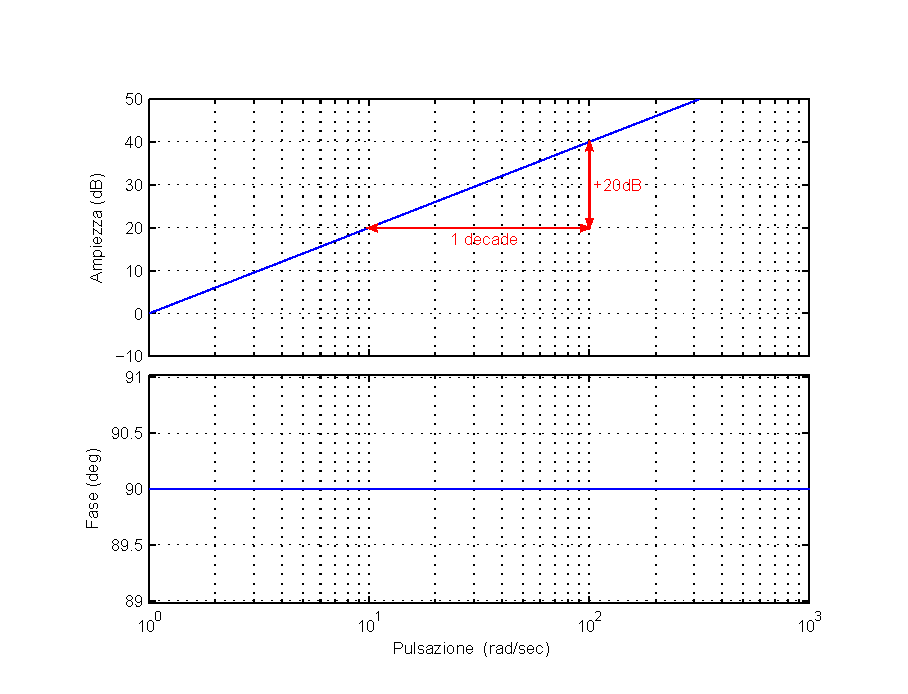
\includegraphics[scale=.7]{eps/zero0}
\caption{Diagrammi di Bode di $H(\jmath\omega)=\jmath\omega$}
\label{fig:zero0}
\end{figure}
\begin{figure}
\centering
\includegraphics[scale=.7]{eps/pole0}
\caption{Diagrammi di Bode di $H(\jmath\omega)=\frac{1}{\jmath\omega}$}
\label{fig:pole0}
\end{figure}

\subsubsection{Zeri destri e sinistri}

Analizziamo il caso in cui la FdT sia del tipo:

\begin{equation*}
H(s)=1\pm s\tau
\end{equation*}

Il modulo sar� uguale sia per zeri destri che sinistri poich� le due FdT sono l'una il complesso coniugato dell'altra:

\begin{equation*}
\begin{split}
A(\omega)	& =\abs{H(\jmath\omega)}_{\dB}=20\Log\abs{1\pm\jmath\omega\tau}= \\
			& =20\Logb{\sqrt{1+\omega^2\tau^2}}=
\begin{cases}
	0\dB & \text{se $\omega\tau\ll 1$} \\
	+3\dB & \text{se $\omega = \frac{1}{\tau}$} \\
	20\Logb{\omega\tau} & \text{se $\omega\tau\gg 1$}
\end{cases}
\end{split}
\end{equation*}

Cio� uno zero non altera il modulo per pulsazioni molto minori di $\frac{1}{\tau}$ e aumenta di $20\dB$ per ogni aumento di una decade della pulsazione (pendenza $+20\dBd$) per pulsazioni molto maggiori di $\frac{1}{\tau}$. La pulsazione $\omega_t=\frac{1}{\tau}$ viene detta \emph{pulsazione di taglio}. In questa pulsazione, il guadagno vale $3\dB$.
La fase di uno zero pu� essere cos� ricavata:

\begin{equation*}
\Phi(\omega)=\Arg{H(\jmath\omega)}=\Arg{1\pm\jmath\omega}=\arctan(\pm\jmath\omega)=\pm\arctan(\jmath\omega)
\end{equation*}

Distinguendo con $\Phi_-(\omega)$ l'argomento del polo sinistro $(1+s\tau)$ e con $\Phi_+(\omega)$ l'argomento del polo destro $(1-s\tau)$:

\begin{gather*}
\Phi_+(\omega)=-\arctan(\omega\tau)=
\begin{cases}
0�		& \text{se $\omega\rightarrow 0$} \\
-45�	& \text{se $\omega=\frac{1}{\tau}$} \\
-90		& \text{se $\omega\rightarrow\infty$}
\end{cases} \\
\Phi_-(\omega)=\arctan(\omega\tau)=
\begin{cases}
0�		& \text{se $\omega\rightarrow 0$} \\
+45�	& \text{se $\omega=\frac{1}{\tau}$} \\
+90		& \text{se $\omega\rightarrow\infty$}
\end{cases}
\end{gather*}

In figura \ref{bode:zero1} sono mostrati i diagrammi di Bode di entrambe le funzioni, lo zero sinistro in blu e quello destro in verde. Le linee tratteggiate sono i diagrammi \emph{reali} mentre quelle continue sono i diagrammi \emph{asintotici}. Faremo pi� spesso utilizzo di questi ultimi, affidabili per� solo per \emph{pulsazioni lontane da quelle di taglio}. In particolare si fa notare che nella pulsazione di taglio l'errore tra il grafico asintotico e quello reale vale $3\dB$.

\begin{figure}
\centering
\includegraphics[scale=.7]{eps/zero1}
\caption{Diagrammi di Bode di $H(\jmath\omega)=1\pm\jmath10\omega$}
\label{bode:zero1}
\end{figure}

\subsubsection{Poli destri e sinistri}
Si prenda ora in esame il caso, simile al precedente, in cui:
\begin{equation*}
H(s)=\dfrac{1}{1\pm s\tau}
\end{equation*}

Calcoliamo analogamente il modulo della funzione, osservando che anche in questo caso � indifferente che si tratti di un polo destro o sinistro.
\begin{equation*}
\begin{split}
A(\omega)	&= \abs{H(\jmath\omega)}_{\dB} = 20\Log\abs*{\dfrac{1}{1\pm\jmath\omega\tau}} = \\
			&= 20\Logb{\frac{1}{\sqrt{1+\omega^2\tau^2}}} =
			\begin{cases}
				0\dB & \text{se $\omega\tau\ll 1$} \\
				-3\dB & \text{se $\omega = \frac{1}{\tau}$} \\
				-20\Logb{\omega\tau} & \text{se $\omega\tau\gg 1$}
			\end{cases}
\end{split}
\end{equation*}
Il comportamento del modulo di un polo, che sia destro o sinistro, � l'opposto d quello di uno zero, procedendo per pulsazioni pi� grandi di quella di taglio con un pendenza di $-20\dBd$. Con le stesse convenzioni del caso precedente, calcoliamo le fasi nei due casi.
\begin{gather*}
\Phi(\omega)=\Arg{H(\jmath\omega)}=\Arg{\frac{1}{1\pm\jmath\omega}}=\Arg{1}-\Arg{1\pm\jmath\omega}=-\Arg{1\pm\jmath\omega} \\
\Phi_+(\omega)=\arctan(\omega\tau)=
\begin{cases}
0�		& \text{se $\omega\rightarrow 0$} \\
+45�	& \text{se $\omega=\frac{1}{\tau}$} \\
+90		& \text{se $\omega\rightarrow\infty$}
\end{cases} \\
\Phi_-(\omega)=-\arctan(\omega\tau)=
\begin{cases}
0�		& \text{se $\omega\rightarrow 0$} \\
-45�	& \text{se $\omega=\frac{1}{\tau}$} \\
-90		& \text{se $\omega\rightarrow\infty$}
\end{cases}
\end{gather*}

In figura \ref{bode:pole1} sono mostrati i diagrammi di Bode del polo sinistro (in blu) e del polo destro (in verde). Le linee tratteggiate sono i diagrammi \emph{reali} mentre quelle continue sono i diagrammi \emph{asintotici}. Si fa notare che nella pulsazione di taglio l'errore tra il grafico asintotico e quello reale vale $-3\dB$.

\begin{figure}

\centering
\includegraphics[scale=.7]{eps/pole1}
\caption{Diagrammi di Bode di $H(\jmath\omega)=\frac{1}{1\pm\jmath10\omega}$}
\label{bode:pole1}
\end{figure}

\subsubsection{Poli e zeri del second'ordine}

I termini del second'ordine sono analiticamente pi� laboriosi da trattare. Tratteremo con precisione solo il caso dello zero del second'ordine mentre il polo del second'ordine sar� dedotto semplicemente dalle seguenti considerazioni (derivate dalle propriet� dei logaritmi e dell'arcotangente):
\begin{align*}
\abs*{\dfrac{1}{H(\jmath\omega)}}_{\dB} & = -\abs*{H(\jmath\omega)}_{\dB} \\
\Arg{\dfrac{1}{H(\jmath\omega)}} & = -\Arg{H(\jmath\omega)}
\end{align*}
Consideriamo ora la FdT con un polo del second'ordine:
\begin{equation*}
H(s)=\left(\dfrac{s}{\omega_z}\right)^2+\dfrac{s}{Q_z\omega_z}+1
\end{equation*}
Ci occuperemo separatamente del calcolo del modulo della FdT. Operando la sostituzione $s=\jmath\omega$ si ottiene la risposta in frequenza:
\begin{equation*}
H(\jmath\omega)=-\left(\dfrac{\omega}{\omega_z}\right)^2+\jmath\dfrac{\omega}{Q_z\omega_z}+1
\end{equation*}
Calcoliamo quindi il modulo in decibel della risposta in frequenza:
\begin{equation*}
\begin{split}
\abs*{H(\jmath\omega)}_{\dB}&=20\Log\abs*{\left(1-\dfrac{\omega^2}{\omega_z^2}\right)+\jmath\dfrac{\omega}{Q_z\omega_z}}=\\&=10\Log\left[\left(1-\dfrac{\omega^2}{\omega_z^2}\right)^2+\dfrac{\omega^2}{Q_z^2\omega_z^2}\right]=
\begin{cases}
0\dB				& \text{se $\omega\rightarrow 0$} \\
-20\Log\abs{Q_z}	& \text{se $\omega=\omega_z$} \\
40\Log(\omega)		& \text{se $\omega\rightarrow\infty$}
\end{cases}
\end{split}
\end{equation*}
Per frequenze lontane dalla \emph{pulsazione di risonanza} $\omega_z$ il comportamento � quello che si avrebbe sovrapponendo due zeri del primo ordine: non vi sono cambiamenti di modulo prima della pulsazione di risonanza e a pulsazioni maggiori di essa si perdono $40\dB$ ogni decade. Il comportamento singolare avviene a frequenze prossime ad $\omega_z$, dove il modulo dipende fortemente dal valore di $Q_z$.
Si fa notare che nel caso in cui: $$Q_z=\frac{1}{2}$$
Si hanno due zeri reali e la FdT potrebbe essere riscritta come:
\begin{equation*}
H(s)=\left(\dfrac{s}{\omega_z}\right)^2+2\dfrac{2}{\omega_z}+1=\left(\dfrac{s}{\omega_z}+4\right)^2
\end{equation*}
Il grafico in blu in figura \ref{bode:zero2amp+} mostra come l'errore nella pulsazione di risonanza � di $+6\dB$, cio� la sovrapposizione di due errori di $+3\dB$ dovuti ai due poli coincidenti.
Per valori maggiori del parametro $Q_z$ si ha un \emph{picco di risonanza} in prossimita di $\omega_z$, pi� vicino a questa frequenza quanto pi� � alto il valore di $Q_z$.

\begin{figure}
\centering
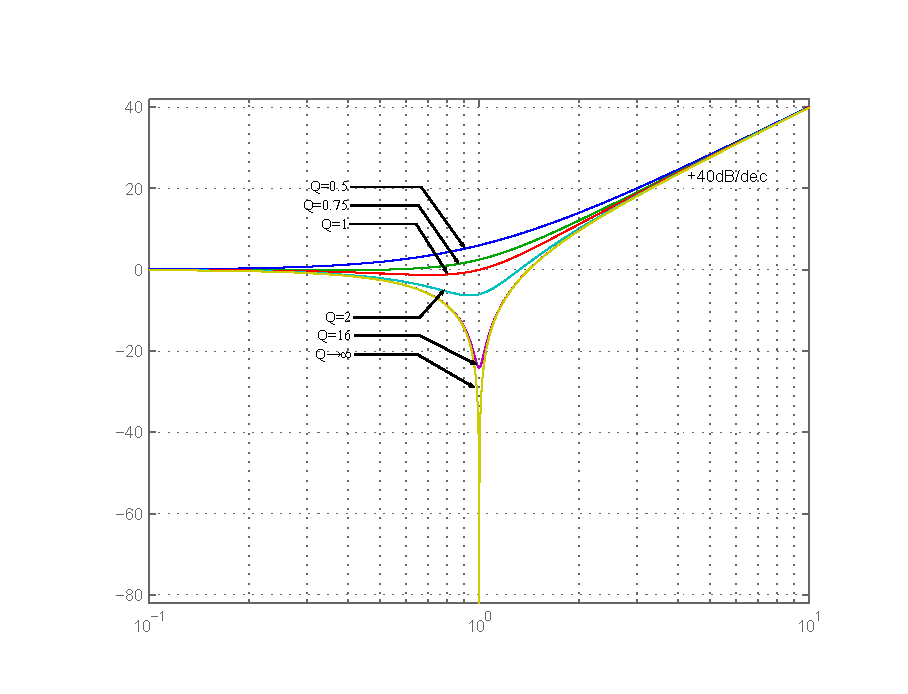
\includegraphics[scale=.7]{eps/zero2amp+}
\caption{Diagrammi di Bode di $H(\jmath\omega)=s^2+2s+1$, con $\omega_z=1$}
\label{bode:zero2amp+}
\end{figure}

La pulsazione $\omega_{max}$ in cui si ha il picco maggiore (in valore assoluto) si pu� calcolare derivando $\abs*{H(\jmath\omega)}$ lungo la variabile $\omega$ e il suo valore assoluto e si pu� quindi trovare il suo valore $A_{max}=\abs*{H(\jmath\omega_{max})}$
\footnote{Verranno omessi i calcoli intermedi che, seppur semplici, sono alquanto laboriosi}:
\begin{gather*}
\omega_{max}=\Set{\omega\in\R^+ | \dfrac{d}{d\omega}\left[\left(1-\dfrac{\omega^2}{\omega_z^2}\right)+\dfrac{\omega}{\omega_z^2 Q_z^2}\right]=0}=\omega_z\sqrt{\dfrac{2Q_z^2-1}{2Q_z^2}} \\
A_{max}=\abs*{H(\jmath\omega_{max})}_{\dB}=-10\Logb{\dfrac{4Q_z^2-1}{4Q_z^2}}
\end{gather*}
Si noti inoltre che per $Q_z\gg 1$ si ha:
$$
\omega_{max}\approx\omega_z	\qquad	A_{max}\approx-20\Log\abs{Q_z}
$$
In figura \ref{bode:zero2amp+} sono mostrati i comportamenti per differenti valori di $Q_z$.

Per quanto riguardo il calcolo della fase della funzione, il procedimento � pi� complesso. Ricordando la definizione di fase \ref{eq:modpha}, vedremo che sar� importante tener conto del segno della parte reale e immaginaria della FdT.
\begin{gather*}
\Re[H(\jmath\omega)]=1-\dfrac{\omega^2}{\omega_z^2} \\
\Im[H(\jmath\omega)]=\dfrac{\omega}{Q_z \omega_z} \\
\Re[H(\jmath\omega)]>=0 \Rightarrow \omega<\omega_z \\
\Im[H(\jmath\omega)]>0 \Rightarrow Q_z>0
\end{gather*}
Possiamo quindi osservare che:
\begin{equation*}
\sgn(\Im[H(\jmath\omega)])=\sgn(Q_z)
\end{equation*}
E inoltre sar� utile calcolare l'arcotangente del rapporto tra parte immaginaria e parte reale:
\begin{equation*}
\begin{split}
\arctan\left(\dfrac{\Im[H(\jmath\omega)]}{\Re[H(\jmath\omega)]}\right) &= 
\arctan\left(\dfrac{\frac{\omega}{Q_z\omega_z}}{1-\frac{\omega^2}{\omega_z^2}}\right) =
\arctan\left(\dfrac{\omega}{Q_z\omega_z}\dfrac{\omega_z^2}{\omega_z^2 - \omega^2}\right) = \\
&= \arctan\left(\dfrac{\omega\omega_z}{Q_z(\omega_z^2 - \omega^2)}\right)
\end{split}
\end{equation*}


\end{document}
